\documentclass[ma3408.tex]{subfiles}
\begin{document}
\chapter{Spectral sequences}
Spectral sequences are a powerful computation tool in topology. Computing with spectral sequences is a bit like computing integral in calculus; it is helpful to have ingenuity and a big bag of tricks - and even that may not be enough! 
\section{Filtered complexes}
We begin our discussion on spectral sequences by discussing filtered complexes. 
\begin{Rem}
Let $C_{\bullet}$ be a chain complex and $F_0C_{\bullet}$ a sub-complex. Then we have a short exact sequence 
\[
0 \to F_0C_{\bullet} \to C_{\bullet} \to C_{\bullet}/F_0C_{\bullet} \to 0
\]
which gives rise to a long exact sequence in homology 
\[
\cdots \to H_i(F_0C_{\bullet}) \to H_i(C_{\bullet}) \to H_i(C_{\bullet}/F_0C_{\bullet}) \xrightarrow{\partial} H_{i-1}(F_0C_{\bullet}) \to \cdots
\]
Suppose we know $H_*(F_0C_{\bullet})$ and $H_*(C_{\bullet}/F_0C_{\bullet})$. Can we compute $H_*(C_{\bullet})$? We can split the long exact sequence into short exact sequences 
\[
0 \to \coker(\partial) \to H_*(C_{\bullet}) \to \ker(\partial) \to 0 
\]
which gives the following procedure for computing $H_*(C_{\bullet})$:
\begin{enumerate}
	\item Compute $H_*(F_0C_{\bullet})$ and $H_*(C_{\bullet}/F_0C_{\bullet})$
	\item Consider the two-term chain complex
\[
H_*(C_{\bullet}/F_0C_{\bullet}) \xrightarrow{\partial} H_*(F_0C_{\bullet}).
\]
Denote its homology groups by $G_1H_*$ and $G_0H_*$. 
\item
There is a short exact sequence
\[
0 \to G_0H_* \to H_*(C_{\bullet}) \to G_1H_* \to 0. 
\]
This determines $H_*(C_{\bullet})$ up to extension.\sidenote{This is a common phenomenon for a spectral sequence. For example, if we have a short exact sequence $0 \to \bbZ/2 \to M \to \bbZ/2 \to 0$, can you say what the middle group is? Not without further information!}
\end{enumerate}
How would we handle the situation if we have a longer filtration: $\cdots F_pC_{\bullet} \subseteq F_{p+1}C_{\bullet} \subseteq \cdots$?

\begin{Exa}
Consider a (semi-simplicial) model of the $2$-sphere $S^2$ with vertices $\{a,b,c\}$, edges $\{A,B,C\}$ and solid triangles $\{P,Q\}$ and with inclusions as soon in \Cref{fig:s2}.\sidenote{This example comes from Example 2.1 of \url{https://arxiv.org/pdf/1702.00666.pdf}.}
\begin{figure}[h!] \centering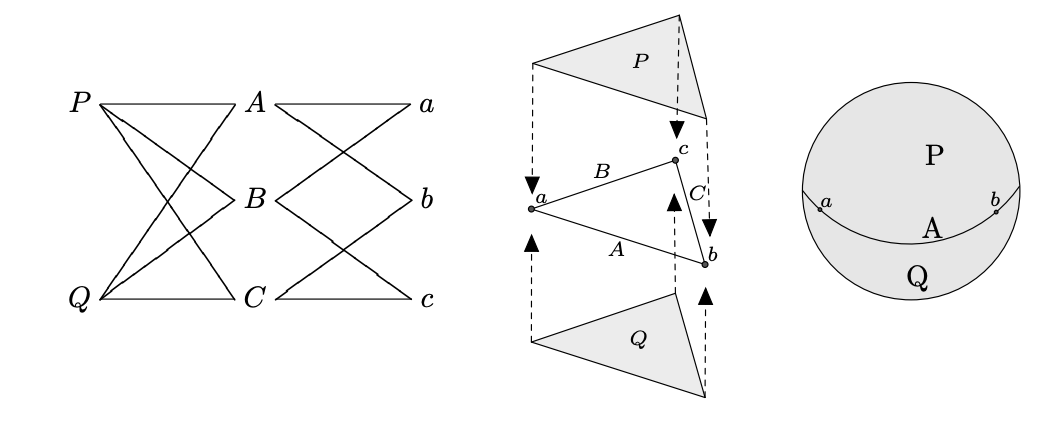
\includegraphics[scale = 0.5]{s2.png}\caption{Simplicial model of $S^2$}\label{fig:s2}\end{figure}
The associated chain complex is $C_{\bullet}$
\[
0 \to \bbZ\{ P, Q\} \xrightarrow{d} \mathbb{Z}\{A,B,C\} \xrightarrow{d} \bbZ\{a,b,c\} \to 0
\]
with
\[
d(P) = C-B+A \quad d(Q) = C-B+A
\]
and
\[
d(A) = b-a \quad d(B) = c-a \quad d(C) = c-b.
\]
One can check directly that $H_i(C_{\bullet};\bbZ) \cong \bbZ$ for $i = 0,2$ and is zero otherwise. Alternatively, we use the following filtration:
\[
\xymatrix@C=10pt@R=0pt{
0\ar[r] &\bbZ\{P,Q\}\ar[r]& \bbZ\{A,B,C\}\ar[r] & \bbZ\{a,b,c\}\ar[r]& 0\\
0\ar[r] &0\ar[r]& \bbZ\{A,B\}\ar[r] & \bbZ\{a,b,c\}\ar[r]& 0\\
0\ar[r] &0\ar[r]& \bbZ\{A\}\ar[r] & \bbZ\{a,b\}\ar[r]& 0.\\
}
\]
The differentials are induced from $d_1$ and $d_2$ and a direct check shows that they are still chain complexes. Passing to the quotient, we get a chain complex we call $E_0$:
\[
\xymatrix@C=10pt@R=0pt{
0\ar[r] &\bbZ\{P,Q\}\ar[r]& \bbZ\{C\}\ar[r] & 0\ar[r]& 0&&d_0(P)=C,d_0(Q)=C\\
0\ar[r] &0\ar[r]& \bbZ\{B\}\ar[r] & \bbZ\{c\}\ar[r]& 0&&d_0(B)=c\\
0\ar[r] &0\ar[r]& \bbZ\{A\}\ar[r] & \bbZ\{a,b\}\ar[r]& 0&&d_0(A)=b-a.\\
}
\]
Taking homology with respect to $d_0$ we obtain $E^1$:
\[
\xymatrix@C=10pt@R=0pt{
0\ar[r] &\bbZ\{P-Q\}\ar[r]& 0 \ar[r] & 0\ar[r]& 0\\
0\ar[r] &0\ar[r]& 0\ar[r] & 0\ar[r]& 0\\
0\ar[r] &0\ar[r]& 0\ar[r] & \bbZ\{\bar a\}\ar[r]& 0.\\
}
\]
The general theory of spectral sequences will tell us that we have computed the homology of $H_*(C_{\bullet})$; there is a $\bbZ$ in degree 2, generated by $P-Q$ and a $\bbZ$ in degree 0, generated by $\bar a$. 
\end{Exa}
\end{Rem}
This leads us to the theory of filtered modules. 
\begin{Def}
	A filtered $R$-module is an $R$-module $A$ together with an increasing sequence of submodules $F_pA \subseteq F_{p+1}A$ indexed by $p \in \mathbb{Z}$ such that $\cup_{p} F_pA = A$ and $\cap_{p} F_pA = \{ 0 \}$. The filtration is bounded if $F_pA = \{ 0 \}$ for $p$ sufficiently small, and $F_pA = A$ for $p$ sufficiently large. The associated graded module is defined by 
	\[
G_pA = F_pA/F_{p-1}A.
	\]
\end{Def}
\begin{Def}
	A filtered chain complex is a chain complex $(C_{\bullet},\partial)$ together with a filtration $\{ F_pC_i \}$ of each $C_i$ such that the differential preserves the filtration: $\partial(F_pC_i) \subseteq F_p C_{i-1}$. Then, $\partial$ induces $\partial \colon G_p C_i \to G_pC_{i-1}$ on the associated graded modules. 
\end{Def}
\begin{Rem}
	The filtration on $C_{\bullet}$ induces a filtration on the homology of $C_{\bullet}$ by
	\[
F_pH_i(C_{\bullet}) = \{ \alpha \in H_i(C_{\bullet}) \mid \exists x \in F_pC_i, \alpha = [x] \}.
	\]
	This has associated graded pieces $G_pH_i(C_{\bullet})$. 
\end{Rem}
\begin{Rem}
Suppose we want to compute $H_*(C_{\bullet})$ and that we can compute the homology of the associated graded pieces $H_*(G_pC_{\bullet})$. Does this determine $G_pH_*(C_{\bullet})$? This leads to the idea of the spectral sequence of a filtered complex. 
\end{Rem}
\section{The spectral sequence of a filtered complex}
\begin{Def}
Let $(F_pC_{\bullet},\partial)$ be a filtered chain complex. Let us write
\[
E^0_{p,q} \coloneqq G_pC_{p+q} = F_pC_{p+q}/F_{p-1}C_{p+q}.
\]
The differential $\partial$ induces a differential on $E^0$,
\[
\partial_0 \colon E^0_{p,q} \to E^0_{p,q-1}.
\]
We denote the homology of the associated graded by
\[
E^1_{p,q} \coloneqq H_{p+q}(G_pC_{\bullet},\partial_0).
\]
\end{Def}
\begin{Rem}
We can think of $E^1_{p,q}$ as a "first order approximation" to $H_*(C_{\bullet})$. We can also define a differential
\[
\partial_1 \colon E^1_{p,q} \to E^1_{p-1,q}
\]
as follows: a homology class $\alpha \in E^1_{p,q}$ can be represented by a chain $x \in F_pC_{p+1}$ such that $\partial x \in F_{p-1}C_{p+q-1}$. We define $\partial_1(\alpha) = [\partial x]$. Because $\partial^2 = 0$, we can check that $\partial_1^2 = 0$ and that $\partial_1$ is well defined. 
\end{Rem}
\begin{Def}
With notation as above, we define
\[
E_2^{p,q} = \ker(\partial_1 \colon E^1_{p,q} \to E^1_{p-1,q})/\im(\partial_1 \colon E^1_{p+1,q} \to E^1_{p,q}). 
\]
\end{Def}
\begin{Rem}
We can continue this procedure, and define an "r"-th order approximation to $G_pH_{p+q}(C_{\bullet})$ by
\[
E^r_{p,q} = \frac{x \in F_pC_{p+q} \mid \partial x \in F_{p-r}C_{p+q-1}}{F_{p-1}C_{p+q} + \partial(F_{p+r-1}C_{p+q+1}}).
\]
The notation denotes the quotient of the numerator by the intersection with the denominator. 

So instead of considering cycles, we consider chains in $F_p$ whose differentials vanishes "to order r", and instead of modding out by the entire image, we only mod out by $\partial(F_{p+r-1})$. 
\end{Rem}
The main result regarding these groups is the following. 
\begin{Lem}\label{lem:ss_filtered_complex}
Let $(F_pC_{\bullet},\partial)$ denote a filtered chain complex, and define $E^r_{p,q}$ as above. Then,
\begin{enumerate}
	\item $\partial$ induces a map 
	\[
\partial_r \colon E^r_{p,q} \to E^r_{p-r,q+r-1}
	\]
	satisfying $\partial_r^2 = 0$. 
	\item $E^{r+1}$ is the homology of the chain complex $(E^r,\partial_r)$, i.e., 
	\[
E^{r+1}_{p,q} = \ker(\partial_r \colon E^r_{p,q} \to E^r_{p-r,q+r-1})/\im(\partial_r \colon E^r_{p+r,q+r-1} \to E^r_{p,q}). 
	\]
	\item $E^1_{p,q} = H_{p+q}(G_pC_{\bullet})$.
	\item If the filtration of $C_i$ is bounded for each $i$, then for every $p,q$ if $r$ is sufficiently large, then 
	\[
E^r_{p,q} = G_pH_{p+q}(C_{\bullet}). 
	\]
\end{enumerate}
\end{Lem}
\begin{proof}
This is a rather tedious diagram chase,\sidenote{For example, see \url{http://www.math.uchicago.edu/~may/MISC/SpecSeqPrimer.pdf}} which generalizes the argument that a short exact sequence of chain complexes induces a long exact sequence on homology. 
\end{proof}
\begin{Exa}
	In this example\sidenote{See page 67 of Mosher--Tangor, \emph{Cohomology Operations and Applications in Homotopy Theory}} we show that the singular and cellular homology groups of a CW-complex $X$ agree. To that end, let $C_*(X)$ denote the singular chain complex of $X$. We filter this by
	\[
F_pC_*(X) \coloneqq C_*(X^p)
	\]
	where $X^p$ denotes the $p$-skeleton of $X$. The associated graded is 
	\[
E^0_{p,q} = C_{p+q}(X^p)/C_{p+q}(X^{p-1}).
	\]
	By definition, the homology is
	\[
E^1_{p,q} = H_{p+q}(X^p,X^{p-1}),
	\]
	the relative homology of the pair $(X^p,X^{p-1})$. 	We have
	\[
H_{p+q}(X^p,X^{p-1})  \cong \begin{cases}
C_p^{cell}(X) & q = 0 \\
0, & q \ne 0
\end{cases}
	\]
	where $C_p^{cell}(X)$ is the cellular chains on $X$, the free $\mathbb{Z}$-module with one generator for each $p$-cell. The cellular differential $\partial \colon C_p^{cell}(X) \to C_{p-1}^{cell}(X)$ is exactly the boundary map $E^1_{p,0} \to E^1_{p-1,0}$. Therefore, we have
	\[
E^2_{p,q} = \begin{cases}
	H_p^{cell}(X), & q = 0 \\
	0, &q \ne 0. 
\end{cases}
	\]
	We must have $\partial_r = 0$ for $r \ge 2$ as either the domain or the range is zero. So, $E_r^{p,q} = E^2_{p,q}$ for all $r \ge 2$. If $X$ is finite-dimensional, then the filtration is bounded and so $H_p(X) = H_p^{cell}(X)$ by \Cref{lem:ss_filtered_complex}.\sidenote{One can allow arbitrary $X$ by, for example, using colimits.}
\end{Exa}
\section{Homological spectral sequences}
We have managed to so far avoid defining exactly what a spectral sequence is. Let us change that now. 
\begin{Def}
	A (homological) spectral sequence is a sequence
	\[
\{E^r_{*,*}, d^r_{*,*} \}_{r \ge 0}
	\]
	of chain complexes of abelian groups, such that
	\[
E^{r+1}_{*,*} = H_*(E^r_{*,*})
	\]
	where the homology is taken with respect to maps (called differentials)
	\[
d^r_{p,q} \colon E^r_{p,q} \to E^r_{p-r,q+r-1}
	\]
	such that $(d^r)^2 = 0$. 
\end{Def}
\begin{Rem}
We say that a spectral sequence is first quadrant if $E^r_{p,q} = 0$ whenever $p < 0$ or $q < 0$. Note that this implies that $d^r_{p,q} = 0$ for $r \gg 0$ (as either the source or the target is zero). In particular,
\[
E^r_{p,q} = E^{r+1}_{p,q} = \cdots = E^{\infty}_{p,q}.
\]
We say that the spectral sequence collapses or degenerates at $E^r$. 

\begin{figure}[h!] \centering\


\tikzset{every picture/.style={line width=0.75pt}} %set default line width to 0.75pt        

\begin{tikzpicture}[x=0.75pt,y=0.75pt,yscale=-1,xscale=1]
%uncomment if require: \path (0,300); %set diagram left start at 0, and has height of 300

%Shape: Axis 2D [id:dp7426994972048953] 
\draw  (50,269) -- (326.5,269)(77.5,56) -- (77.5,295) (319.5,264) -- (326.5,269) -- (319.5,274) (72.5,63) -- (77.5,56) -- (82.5,63)  ;
%Straight Lines [id:da5492274811444786] 
\draw    (271.39,211.44) -- (307.75,249) ;
\draw [shift={(270,210)}, rotate = 45.93] [color={rgb, 255:red, 0; green, 0; blue, 0 }  ][line width=0.75]    (10.93,-3.29) .. controls (6.95,-1.4) and (3.31,-0.3) .. (0,0) .. controls (3.31,0.3) and (6.95,1.4) .. (10.93,3.29)   ;
%Straight Lines [id:da25964752287559123] 
\draw    (202.92,143.41) -- (270,210) ;
\draw [shift={(201.5,142)}, rotate = 44.79] [color={rgb, 255:red, 0; green, 0; blue, 0 }  ][line width=0.75]    (10.93,-3.29) .. controls (6.95,-1.4) and (3.31,-0.3) .. (0,0) .. controls (3.31,0.3) and (6.95,1.4) .. (10.93,3.29)   ;
%Straight Lines [id:da7644752936176098] 
\draw    (147.42,88.41) -- (201.5,142) ;
\draw [shift={(146,87)}, rotate = 44.74] [color={rgb, 255:red, 0; green, 0; blue, 0 }  ][line width=0.75]    (10.93,-3.29) .. controls (6.95,-1.4) and (3.31,-0.3) .. (0,0) .. controls (3.31,0.3) and (6.95,1.4) .. (10.93,3.29)   ;
%Straight Lines [id:da1914423583168492] 
\draw  [dash pattern={on 4.5pt off 4.5pt}]  (201.5,142) -- (200.5,273) ;
%Straight Lines [id:da5743726994033245] 
\draw  [dash pattern={on 4.5pt off 4.5pt}]  (77.5,141) -- (201.5,142) ;
%Straight Lines [id:da7967677178497095] 
\draw  [dash pattern={on 4.5pt off 4.5pt}]  (270,210) -- (270,270) ;
%Straight Lines [id:da8691680032874185] 
\draw  [dash pattern={on 4.5pt off 4.5pt}]  (80,210) -- (270,210) ;

% Text Node
\draw (79.65,274.1) node [anchor=north west][inner sep=0.75pt]   [align=left] {0};
% Text Node
\draw (261,186.4) node [anchor=north west][inner sep=0.75pt]    {$E_{p,q}^{r}$};
% Text Node
\draw (191,116.4) node [anchor=north west][inner sep=0.75pt]    {$E_{p-r,q+r-1}^{r}$};
% Text Node
\draw (285,204.4) node [anchor=north west][inner sep=0.75pt]    {$d^{r}$};
% Text Node
\draw (229,151.4) node [anchor=north west][inner sep=0.75pt]    {$d^{r}$};
% Text Node
\draw (171,80.4) node [anchor=north west][inner sep=0.75pt]    {$d^{r}$};
% Text Node
\draw (184,275.4) node [anchor=north west][inner sep=0.75pt]    {$p-r$};
% Text Node
\draw (14,133.4) node [anchor=north west][inner sep=0.75pt]    {$q+r-1$};
% Text Node
\draw (60,203.4) node [anchor=north west][inner sep=0.75pt]    {$q$};
% Text Node
\draw (261,275.4) node [anchor=north west][inner sep=0.75pt]    {$p$};
\end{tikzpicture}
\caption{The $E^r$-page of a homological spectral sequence}
\end{figure}
\end{Rem}
\begin{Def}
	If $\{H_n\}_{n}$ are groups, then we say that the spectral sequence converges, or abuts, to $H_*$, denoted $E^2_{*,*} \implies H_*$, if for each $n$ there is a filtration
	\[
H_n = D_{n,0} \subseteq D_{n-1,1} \subseteq \cdots \subseteq D_{1,n-1} \subseteq D_{0,n} \subseteq 0
	\]
	such that, for all $p,q$, 
	\[
E^{\infty}_{p,q} = D_{p,q}/D_{p-1,q+1}.
	\]
\end{Def}
\begin{Rem}
In more straightforward terms: the if we look along the $n$-th diagonal of the spectral sequence, then the $E_{\infty}$-page computes the associated graded of the filtration on $H_n$. For example, if $E^{\infty}_{p,q} = 0$ for all $p+q =n$, then $H_n = 0$. If there is only a single non-zero term, say $E^{\infty}_{p,n-p}$, then the filtration is trivial, and $H_n = E^{\infty}_{p,n-p}$. If we have two non-zero terms, then $H_n$ fits into a short exact sequence, and so on. 
\end{Rem}
\begin{Exa}\label{ex:ss_filtered_complex}
We have previously discussed the spectral sequence of a filtered complex without explicitly mentioning it. Indeed, if $C_{\bullet}$ is a filtered chain complex, then there is a spectral sequence with $E^1_{p,q} = H_{p+q}(G_pC_{\bullet})$, such that if the filtration of $C_i$ is bounded for each $i$ the spectral sequence converges to $H_{p+q}(C_{\bullet})$.\sidenote{Recall what this means: we have $E^{\infty}_{p,q} = G_pH_{p+q}(C_{\bullet})$.}
\end{Exa}
\section{The spectral sequence of a double complex}
An important example where a filtered complex arises is from a double complex. 
\begin{Def}
	A double complex is a bi-indexed family $\{ C_{p,q} \}$ of abelian groups, with two differentials
	\[
d' \colon C_{p,q} \to C_{p-1,q}, \quad d" \colon C_{p,q} \to C_{p,q-1}
	\]
	such that $d'd' = 0, d"d" = 0$, and $d'd" + d"d' = 0$. For simplicity, we also assume that $C_{p,q} = 0$ for $p< 0$ or $q<0$.
\end{Def}
\begin{Exa}\label{exa:double_complex_cc}
Suppose that $(A,d_A)$ and $(B,d_B)$ are chain complexes. If we define $C_{p,q} = A_p \otimes B_q$ and define $d' = d_A \otimes 1$ and $d" = (-1)^p1 \otimes d_B$, then $C_{p,q}$ is a double complex.\sidenote{Try and verify this to make sure you understand the definitions.} 
\end{Exa}
\begin{Cons}
A double complex gives rise to a chain complex (the total complex), defined by $C_n = \sum_{p+q = n} C_{p,q}$ and $d = d' + d"$. This has two obvious filtrations, by row and by column:
\begin{enumerate}
	\item ${}'C^p_n = \sum_{j+q = n, j \le p} C_{j,q}$.
	\item ${}"C^p_n = \sum_{p+q = n, k \le q} C_{p,k}$.
\end{enumerate}
The spectral sequence of a filtered complex (\Cref{ex:ss_filtered_complex}) gives us two spectral sequences:
\begin{enumerate}
	\item ${}'E^1_{p,q} = H_{p+q}('C^p/'C^{p-1}) = C_{p,n-p}$.
	\item ${}"E^1_{p,q} = H_{p+q}("C^q/"C^{q-1}) = C_{q,n-q}$.
\end{enumerate}
One checks that $'E^1$ is computed via means of $d"$ and that $d^1$ is induced by $d'$, while in $"E^1$ the role of the two indices are exchanged. We can therefore write:
\begin{enumerate}
	\item ${}'E^2_{p,q} = H'_pH"_q(C)$.
	\item ${}"E^2_{p,q} = H"_qH'_p(C)$.
\end{enumerate}
Moreover, both spectral sequences converge to $H_*(C)$, and the idea is to compare the two spectral sequences. 
\end{Cons}
It is constructive to do an example. 
\begin{Exa}
Let $'\Tor(A,B)$ be defined as follows: take a free resolution of $A$, $0 \to R' \to F' \to A \to 0$, then $'\Tor(A,B)$ is defined by
\[
0 \to '\Tor(A,B) \to R' \otimes B \to F' \otimes B \to A \otimes B \to 0. 
\]
Similarly, let $"\Tor(A,B)$ be defined as follows: take a free resolution of $B$, $0 \to R" \to F" \to B \to 0$, then $"\Tor(A,B)$ is defined by
\[
0 \to "\Tor(A,B) \to A \otimes R" \to A \otimes F" \to A \otimes B \to 0. 
\]
It is a classical theorem of homological algebra that $\Tor(A,B) = "\Tor(A,B)$. Let us prove this via a spectral sequence argument. 

Let $X$ be the chain complex $0 \to R' \xrightarrow{d'} F' \to 0$ and let $Y$ be the chain complex $0 \to R" \xrightarrow{d"}  F" \to 0$. We can build a double complex $C_{*,*}$ as in \Cref{exa:double_complex_cc}, which we write as a matrix:
\[
\begin{bmatrix}C_{p,q}\end{bmatrix} =  \begin{bmatrix}
F' \otimes R" & R' \otimes R" \\
F' \otimes F" & R' \otimes F" 
\end{bmatrix}  
\]

We have two spectral sequences: the first is take vertical and then horizontal homology:
\[
H_q"(C_{p,q})=  \begin{bmatrix}
"\Tor(F',B) & '\Tor(R',B) \\
F' \otimes B & R' \otimes B
\end{bmatrix}  = \begin{bmatrix}
0 & 0 \\
F' \otimes B & R' \otimes B
\end{bmatrix} 
\]
and
\[
H_pH_q"(C_{p,q}) =  \begin{bmatrix}
0 & 0 \\
A \otimes B & '\Tor(A,B)
\end{bmatrix}
\]

In other words, the total complex has $H_0(C) = A \otimes B$ and $H_1(C) = '\Tor(A,B)$. 

However, we can use the second spectral sequence, which first takes horizontal and then vertical homology: 
\[
H_p(C_{p,q})  \begin{bmatrix}
A \otimes R" & '\Tor(A,R") \\
A \otimes F" & '\Tor(A,F")
\end{bmatrix}  = \begin{bmatrix}
A \otimes R" & 0 \\
A \otimes F" & 0
\end{bmatrix} 
\]
and then
\[
H"_qH_p(C_{p,q}) =  \begin{bmatrix}
"\Tor(A,B) & 0 \\
A \otimes B & 0
\end{bmatrix} \]
In this case we see that $H_0(C) = A \otimes B$ and $H_1(C) = "\Tor(A,B)$. Therefore, $'\Tor(A,B) = "\Tor(A,B)$. 
\end{Exa}
\begin{exercise}{The snake lemma}{}
Show, using spectral sequences, the following result in homological algebra (the snake lemma):

Given a commutative diagram
\[
% https://tikzcd.yichuanshen.de/#N4Igdg9gJgpgziAXAbVABwnAlgFyxMJZABgBpiBdUkANwEMAbAVxiRGJAF9T1Nd9CKAIzkqtRizYBBLjxAZseAkQBMo6vWatEIAEKzeigUQDM68VrYBhA-L5LBJUkLGbJOjt0P9lw564ltECkAclsFH0c1Fw1Atl0wrzsjX2QzGIt3ECtEuQiHIgAWf1jLD3D7YxRiylKszzEYKABzeCJQADMAJwgAWyQREBwIJABWagY6ACMYBgAFSt8QLqxmgAscEDqgjttuvqQ1IZHEADYJ6dmFlMFl1Y2tzKDmvZ7+xDNjpAB2C5n5xa3FbrTbbNhrV4HRBkL6IIRJfbvYqw0YIt4DajDQ5oqHjWGnHHvc6w76Ew6Yk4mMkfClIACc1N+sIAHJwKJwgA
\begin{tikzcd}
0 \arrow[r] & A \arrow[d, "f"'] \arrow[r] & B \arrow[d, "g"'] \arrow[r] & C \arrow[d, "h"'] \arrow[r] & 0 \\
0 \arrow[r] & A' \arrow[r]                & B' \arrow[r]                & C' \arrow[r]                & 0
\end{tikzcd}\]
in an abelian category with exact rows, there is a long exact sequence 
\[
\begin{split}
0 \to \ker(f) \to \ker(g) &\to \ker(h) \\&\to \coker(f) \to \coker(g) \to \coker(h) \to 0. 
\end{split}
\]
\end{exercise}
\begin{exercise}{}{}
(1) Suppose we have a commutative triangle
	% https://q.uiver.app/?q=WzAsMyxbMCwwLCJBIl0sWzIsMCwiQyJdLFsxLDEsIkIiXSxbMCwxLCJpIl0sWzAsMiwiZiIsMl0sWzEsMiwicSJdXQ==
\[\begin{tikzcd}
	A && C \\
	& B
	\arrow["i", from=1-1, to=1-3]
	\arrow["f"', from=1-1, to=2-2]
	\arrow["q", from=1-3, to=2-2]
\end{tikzcd}\]
Show using the snake lemma that 
\[
\ker(\coker f \to \coker q) \cong \im(q)/\im(f) 
\]
and
\[
\quad \coker(\coker f \to \coker q) = 0.
\]

(2) Using Part (1), prove the following `butterfly lemma': given a commutative diagram
% https://q.uiver.app/?q=WzAsNSxbMSwxLCJDIl0sWzAsMCwiQSJdLFswLDIsIkIiXSxbMiwwLCJEIl0sWzIsMiwiRSJdLFsxLDIsImYiLDJdLFsxLDAsImkiXSxbMCwyLCJxIl0sWzMsMCwiaiIsMl0sWzMsNCwiZyJdLFswLDQsInAiLDJdXQ==
\[\begin{tikzcd}
	A && D \\
	& C \\
	B && E
	\arrow["f"', from=1-1, to=3-1]
	\arrow["i", from=1-1, to=2-2]
	\arrow["q", from=2-2, to=3-1]
	\arrow["j"', from=1-3, to=2-2]
	\arrow["g", from=1-3, to=3-3]
	\arrow["p"', from=2-2, to=3-3]
\end{tikzcd}\]

of abelian groups, in which the diagonals $pi$ and $qj$ are exact at $C$, there is an isomorphism
\[
\frac{\im q}{\im f} \cong \frac{\im p}{\im g}. 
\]
\end{exercise}
\section{The Serre spectral sequence}
For us the most important example of a spectral sequence will be the Serre spectral sequence. We will state the theorem now and then return to the proof after some examples and applications. 
\begin{Thm}[The Serre spectral sequence]
Let $\pi \colon E \to F$ be a fibration with fiber $F$ and assume that $\pi_1(B) = 0$ and $\pi_0(F) = 0$, then there is a first quadrant spectral sequence
\[
E^2_{p,q} = H_p(B;H_q(F)) \implies H_{p+q}(E). 
\]
In particular, this means there is a filtration
\[
H_n(E) = D_{n,0} \supseteq D_{n-1,1} \supseteq \ldots \supseteq D_{0,n} \supseteq D_{-1,n+1} = 0
\]
such that $E^{\infty}_{p,q} = D_{p,q}/D_{p-1,q+1}$. 
\end{Thm}
\begin{Rem}
There is a version of this spectral sequence where $\pi_1(B) \ne 0$; the $E_2$-page is then given by the cohomology of $B$ with local coefficients $\mathcal{H}_q(F)$. This will not play a role in this course. 
\end{Rem}
\begin{Exa}\label{ex:hopf_fibration}
Consider the Hopf fibration $S^1 \to S^3 \to S^2$. We have 
\[
E^2_{p,q} = H_p(S^2;H_q(S^1)) \cong \begin{cases}
	\bbZ & p = 0,2 \text{ and } q = 0, 1 \\
	0 & \text{ otherwise.}
\end{cases}
\]
The $E^2$-term is as follows (and we have $E^3 = E^{\infty}$ for degree reasons):
\begin{sseqdata}[ name = basice2,
x label = { $H_*(S^2)$},
y label = { $H_*(S^1)$ },
homological Serre grading, classes = {draw = none } ]
\class["\mathbb{Z}"](0,0)
\class["\mathbb{Z}"](2,0)
\class["\mathbb{Z}"](0,1)
\class["\mathbb{Z}"](2,1)
\class["{}"](3,1)
\class["{}"](0,2)
\d["\cdot n"]2(2,0)
\end{sseqdata}
\printpage[ name = basice2, page = 2 ] 

There are three possibilities for the $d_2$-differential (which is multiplication by $n \in \bbZ$ as indicated): either $n = 0,n= \pm 1$ or $n \ne 0,\pm 1$, which lead to the following $E^3 = E^{\infty}$-page:
\begin{sseqdata}[ name = basice3a, xscale = 0.6,
x label = { $H_*(S^2)$ \\ $n = 0$},
y label = { $H_*(S^1)$ }, homological Serre grading, classes = {draw = none } ]
\class["\mathbb{Z}"](0,0)
\class["\mathbb{Z}"](2,0)
\class["\mathbb{Z}"](0,1)
\class["\mathbb{Z}"](2,1)

\end{sseqdata}
\begin{sseqdata}[ name = basice3b, xscale = 0.6,
x label = { $H_*(S^2)$ \\ $n = \pm 1$},
y label = { $H_*(S^1)$ }, homological Serre grading, classes = {draw = none } ]
\class["\mathbb{Z}"](0,0)
\class["\mathbb{Z}"](2,0)
\class["\mathbb{Z}"](0,1)
\class["\mathbb{Z}"](2,1)
\d["\cdot n"]2(2,0)
\end{sseqdata}
\begin{sseqdata}[ name = basice3c, xscale = 0.6,
x label = { $H_*(S^2)$ \\ $n \ne 0,\pm 1$ },
y label = { $H_*(S^1)$ }, homological Serre grading, classes = {draw = none } ]
\class["\mathbb{Z}"](0,0)
\class["\mathbb{Z}"](2,0)
\class["\mathbb{Z}"](0,1)
\class["\mathbb{Z}"](2,1)
\d["\cdot n"]2(2,0)
\replacetarget["\mathbb{Z}/n"] 
\end{sseqdata}
\noindent \begin{minipage}{0.35\textwidth}
\printpage[ name = basice3a, page = 3 ]   \quad
\end{minipage}
\begin{minipage}{0.35\textwidth}
\printpage[ name = basice3b, page = 3 ]  \quad
\end{minipage}
\begin{minipage}{0.35\textwidth}
\printpage[ name = basice3c, page = 3 ] 
\end{minipage}
We see that taking $n = \pm 1$ computes the correct answer for $H_*(S^3)$; we have a copy of $\bbZ$ in the $p+q= 0$ and $p + q = 3$ columns, as required. 
\end{Exa}
\begin{Exa}
There is a fibration $SU(n-1) \to SU(n) \to S^{2n-1}$. Taking $n = 3$ and using $SU(2) \cong S^3$, we obtain a fibration $S^3 \to SU(3) \to S^5$. We have
\[
E^2_{p,q} \cong \begin{cases}
	\bbZ & p = 0,5 \text{ and } q = 0, 3 \\
	0 & \text{ otherwise.} 
	\end{cases}
\]
The $E^2$-term is as follows:
\begin{sseqdata}[ name = su(3),xscale = 0.6,yscale = 0.6,
x label = { $H_*(S^5)$},
y label = { $H_*(S^3)$ },
homological Serre grading, classes = {draw = none } ]
\class["\mathbb{Z}"](0,0)
\class["\mathbb{Z}"](5,0)
\class["\mathbb{Z}"](0,3)
\class["\mathbb{Z}"](5,3)
\class["{}"](3,1)
\d["d_2"]2(5,0)
\end{sseqdata}
\printpage[ name = su(3), page = 2 ] 

Note that there are no differentials for degree reasons, as shown for $d_2$. Therefore, the spectral sequence collapses and we see that
\[
H_i(SU(3)) \cong \begin{cases}\bbZ, &i = 0,3,5,8 \\ 0, & \text{otherwise.}\end{cases}
\]
\end{Exa}
\begin{Exa}
We can continue the previous example and take $n = 4$ to get a fibration $SU(3) \to SU(4) \to S^7$. We can compute the $E^2$-term using the previous example
\[
E^2_{p,q} = H_p(S^7;H_q(SU(3))) \cong \begin{cases} \bbZ, & p = 0,7, q = 0,3,5,8 \\ 0, &\text{otherwise.}\end{cases}
\]
The $E^2$-term is as follows:
\begin{sseqdata}[ name = su(4),xscale = 0.6, yscale = 0.6,
x label = { $H_*(S^7)$},
y label = { $H_*(SU(3))$ },
homological Serre grading, classes = {draw = none } ]
\class["\mathbb{Z}"](0,0)
\class["\mathbb{Z}"](7,0)
\class["\mathbb{Z}"](0,3)
\class["\mathbb{Z}"](7,3)
\class["\mathbb{Z}"](0,5)
\class["\mathbb{Z}"](7,5)
\class["\mathbb{Z}"](0,8)
\class["\mathbb{Z}"](7,8)
\end{sseqdata}
\printpage[ name = su(4), page = 2 ] 

Note that there are no differentials for degree reasons, and we compute
\[
H_i(SU(4)) \cong \begin{cases}\bbZ, &i = 0,3,5,7,8,10,12,15 \\ 0, & \text{otherwise.}\end{cases}
\]
\end{Exa}
\begin{Rem}
If one tries the same argument for $SU(5)$ there are possible differentials. We will see later that it is easier to use cohomology, where one can use multiplicative structures to rule out differentials. 
\end{Rem}
\begin{Rem}[Naturality of the Serre spectral sequence]\label{Rem:naturality_of_ss}
The Serre spectral sequence is natural in the following sense. Suppose we are given two fibrations satisfying the hypothesis of the Serre spectral sequence, and a map between them: 
% https://q.uiver.app/?q=WzAsNixbMCwwLCJGIl0sWzEsMCwiRSJdLFsyLDAsIkIiXSxbMCwxLCJGJyJdLFsxLDEsIkUnIl0sWzIsMSwiQiciXSxbMCwxLCIiLDAseyJzdHlsZSI6eyJ0YWlsIjp7Im5hbWUiOiJob29rIiwic2lkZSI6InRvcCJ9fX1dLFsxLDJdLFszLDQsIiIsMCx7InN0eWxlIjp7InRhaWwiOnsibmFtZSI6Imhvb2siLCJzaWRlIjoidG9wIn19fV0sWzQsNV0sWzAsM10sWzEsNCwiXFx0aWxkZSBmIl0sWzIsNSwiZiJdXQ==
\[\begin{tikzcd}[ampersand replacement=\&]
	F \& E \& B \\
	{F'} \& {E'} \& {B'}
	\arrow[hook, from=1-1, to=1-2]
	\arrow[from=1-2, to=1-3]
	\arrow[hook, from=2-1, to=2-2]
	\arrow[from=2-2, to=2-3]
	\arrow[from=1-1, to=2-1]
	\arrow["{\tilde f}", from=1-2, to=2-2]
	\arrow["f", from=1-3, to=2-3]
\end{tikzcd}\]
Then the following hold:
\begin{enumerate}
	\item There are induced maps $f_*^r \colon E^r_{p,q} \to 'E^r_{p,q}$ commuting with differentials, i,e, the diagram
% https://q.uiver.app/?q=WzAsNCxbMCwwLCJFXnJfe3AscX0iXSxbMSwwLCJFXnJfe3AtcixxK3ItMX0iXSxbMCwxLCInRV5yX3twLHF9Il0sWzEsMSwiJ0Vecl97cC1yLHErci0xfSJdLFswLDEsImRfciJdLFswLDIsImZecl8qIiwyXSxbMiwzLCInZF9yIiwyXSxbMSwzLCInZl8qXnIiXV0=
\[\begin{tikzcd}[ampersand replacement=\&]
	{E^r_{p,q}} \& {E^r_{p-r,q+r-1}} \\
	{'E^r_{p,q}} \& {'E^r_{p-r,q+r-1}}
	\arrow["{d_r}", from=1-1, to=1-2]
	\arrow["{f^r_*}"', from=1-1, to=2-1]
	\arrow["{'d_r}"', from=2-1, to=2-2]
	\arrow["{f_*^r}", from=1-2, to=2-2]
\end{tikzcd}\]
	commutes, and moreover  $f_*^{r+1}$ is the map induced on homology by $f_*^r$.
	\item The map $\tilde f_* \colon H_*(E) \to H_*(E')$ preserves filtrations, inducing a map on associated graded which is exactly $f_*^{\infty}$. 
	\item Under the isomorphisms $E^2_{p,q} \cong H_p(B;H_q(F))$ and $'E^2_{p,q} \cong H_p(B';H_q(F'))$ the map $f_*^2$ corresponds to the map induced by the maps $B \to B'$ and $F \to F'$. 
\end{enumerate}
\end{Rem}
Once again, we can demonstrate this with an example. 
\begin{Exa}
We recall the Hopf fibration $S^1 \to S^3 \to S^2$. This factors through $\bbR P^3 = S^3/\{ \pm 1 \}$ as in the following diagram:
% https://q.uiver.app/?q=WzAsNixbMCwwLCJTXjEiXSxbMSwwLCJTXjMiXSxbMiwwLCJTXjIiXSxbMCwxLCJTXjEvXFx7IFxccG0gMSBcXH0iXSxbMSwxLCJTXjMvXFx7IFxccG0gMVxcfSJdLFsyLDEsIlNeMiJdLFswLDEsIiIsMCx7InN0eWxlIjp7InRhaWwiOnsibmFtZSI6Imhvb2siLCJzaWRlIjoidG9wIn19fV0sWzEsMl0sWzAsMywicSIsMix7InN0eWxlIjp7ImhlYWQiOnsibmFtZSI6ImVwaSJ9fX1dLFsxLDQsInEiLDIseyJzdHlsZSI6eyJoZWFkIjp7Im5hbWUiOiJlcGkifX19XSxbMyw0LCIiLDEseyJzdHlsZSI6eyJ0YWlsIjp7Im5hbWUiOiJob29rIiwic2lkZSI6InRvcCJ9fX1dLFs0LDVdLFsyLDUsIiIsMSx7ImxldmVsIjoyLCJzdHlsZSI6eyJoZWFkIjp7Im5hbWUiOiJub25lIn19fV1d
\[\begin{tikzcd}[ampersand replacement=\&]
	{S^1} \& {S^3} \& {S^2} \\
	{S^1/\{ \pm 1 \}} \& {S^3/\{ \pm 1\}} \& {S^2}
	\arrow[hook, from=1-1, to=1-2]
	\arrow[from=1-2, to=1-3]
	\arrow["q"', two heads, from=1-1, to=2-1]
	\arrow["q"', two heads, from=1-2, to=2-2]
	\arrow[hook, from=2-1, to=2-2]
	\arrow[from=2-2, to=2-3]
	\arrow[Rightarrow, no head, from=1-3, to=2-3]
\end{tikzcd}\]
We see that we have a fibration $S^1 \to \bbR P^3 \to S^2$. The $'E^2$-term of this spectral sequence is as for the Hopf fibration:
\[
E^2_{p,q} = H_p(S^2;H_q(S^1)) \cong \begin{cases}
	\bbZ & p = 0,2 \text{ and } q = 0, 1 \\
	0 & \text{ otherwise.}
\end{cases}
\]
As in \Cref{ex:hopf_fibration} there is only one possible differential, which is $'d_2 \colon 'E^2_{2,0} \to 'E^2_{0,1}$, and this is given by multiplication by an integer $n$. We use naturality to determine what this is. We note that we have a commutative diagram
\[\begin{tikzcd}[ampersand replacement=\&]
	{H_2(S^2;H_0(S^1))} \& H_0(S^2;H_1(S^1)) \\
	{H_2(S^2;H_0(S^1/\{ \pm 1\}))} \& H_0(S^2;H_1(S^1/\{ \pm 1\})) \\
	\arrow["{d_2}", "\cong"', from=1-1, to=1-2]
	\arrow["{q_*}"', "\cong", from=1-1, to=2-1]
	\arrow["{'d_2}"', from=2-1, to=2-2]
	\arrow["{\cdot 2}", from=1-2, to=2-2]
\end{tikzcd}\]
The right hand arrow is multiplication by 2 because the map induced on homology by $S^1 \to S^1/\{ \pm 1 \}$ has degree 2 (it is the attaching map for the top cell of $\bbR P^2$). Commutativity of the diagram implies that $'d_2$ is multiplication by 2. Therefore, the $E^2$ and $E^3= E^{\infty}$-terms are as follows:
\begin{sseqdata}[ name = rp3,
x label = { $H_*(S^2)$},
y label = { $H_*(S^1)$ },
homological Serre grading, classes = {draw = none } ]
\class["\mathbb{Z}"](0,0)
\class["\mathbb{Z}"](2,0)
\class["\mathbb{Z}"](0,1)
\class["\mathbb{Z}"](2,1)
\class["{}"](3,1)
\class["{}"](0,2)
\d["\cdot 2"]2(2,0)
\replacetarget["\mathbb{Z}/2"] 
\end{sseqdata}
 \begin{minipage}{0.5\textwidth}
\printpage[ name = rp3, page = 2 ] \quad 
\end{minipage}
 \begin{minipage}{0.5\textwidth}
\printpage[ name = rp3, page = 3 ] \quad
\end{minipage}
We deduce that
\[
H_i(\bbR P^3) \cong \begin{cases} \bbZ, &i = 0,3 \\ \bbZ/2, & i = 1 \\ 0, &\text{otherwise.}\end{cases}
\]
\end{Exa}
\begin{Rem}
It is also possible to deduce some information about $H^*(F)$ or $H^*(B)$ in certain cases, as the following example demonstrates. 
\end{Rem}
\begin{Exa}\label{ex:s_infty}
There is a fibration $S^1 \to S^{\infty} \to \bbC P^{\infty}$. Note that $\pi_1(\bbC P^{\infty}) = 0$, so we can run the Serre spectral sequence. We have
\[
E^2_{p,q} = \begin{cases} H_p(\bbC P^{\infty}), & q = 0,1 \\ 0, &\text{otherwise.}\end{cases} 
\]
We also know that the spectral sequence converges to $H_{p+q}(S^{\infty},\bbZ)$, which is only non-zero when $p+q = 0$. In particular, the $E^{\infty}$ page should be zero except for $E^{\infty}_{0,0}$. Now consider the $E_2$-page of the spectral sequence:
\begin{sseqdata}[ name = sinfty,xscale = 2, x axis extend end=1cm,
x label = { $H_*(\bbC P^{\infty})$},
y label = { $H_*(S^1)$ },
homological Serre grading, classes = {draw = none } ]
\class["\bbZ"](0,0)
\class["H_1(\bbC P^{\infty})"](1,0)
\class["H_2(\bbC P^{\infty})"](2,0)
\class["H_3(\bbC P^{\infty})"](3,0)
\class["\bbZ"](0,1)
\class["H_1(\bbC P^{\infty})"](1,1)
\class["H_2(\bbC P^{\infty})"](2,1) 
\class["H_3(\bbC P^{\infty})"](3,1)
\class["{}"](0,2)
\d[]2(2,0)
\d[]2(3,0)
\end{sseqdata}
\printpage[ name = sinfty, page = 2 ] 

\noindent Note that for degree reasons $E^2_{1,0} \cong H_1(\bbC P^{\infty})$ survives the spectral sequences, and so must be 0. So the $E^2$-page is as follows:
\begin{sseqdata}[ name = sinfty2,xscale = 2,x axis extend end=1cm,
x label = { $H_*(\bbC P^{\infty})$},
y label = { $H_*(S^1)$ },
homological Serre grading, classes = {draw = none } ]
\class["\bbZ"](0,0)
\class["H_2(\bbC P^{\infty})"](2,0)
\class["H_3(\bbC P^{\infty})"](3,0)
\class["\bbZ"](0,1)
\class["0"](1,1)
\class["0"](1,0)
\class["H_2(\bbC P^{\infty})"](2,1) 
\class["H_3(\bbC P^{\infty})"](3,1)
\class["{}"](0,2)
\d[]2(2,0)
\d[]2(3,0)
\end{sseqdata}
\printpage[ name = sinfty2, page = 2 ] 

\noindent By the same argument $E^2_{3,0} \cong H_3(\bbC P^{\infty})$ survives the spectral sequences, and so must be 0. Inductively, we deduce that $H_n(\bbC P^{\infty}) = 0$ for all $n$ odd. Since $E^2_{0,1} \cong \bbZ$ must also die in the spectral sequence, we see that we must have $H_2(\bbC P^{\infty}) \cong \bbZ$, and that $d^2$ must be an isomorphism. Continuing inductively, we get
\[
H_n(\bbC P^{\infty}) \cong \begin{cases} \bbZ, & n \text{ even}\\  \bbZ, & 0 \text{ odd.}\end{cases}
\]
\end{Exa}

\begin{Exa}\label{ex:loop_spaces}
In our next example, we compute $H_*(\Omega S^n)$ for $n >1 $. We use the path-space fibration of \Cref{rem:path_space_fibration}. In this case, this takes the form
\[
\Omega S^n \to PS^n \to S^n
\]
where we recall that $PS^n$ is contractible, i.e. $H_0(PS^n) = \bbZ$ and is zero otherwise. In particular, the only non-zero term on the $E^{\infty}$-page of the spectral sequence is a copy of $\bbZ$ when $p+q = 0$. Now consider a small portion of the $E_2$-term:
\begin{sseqdata}[name = loop_sphere_s2,no x ticks,no y ticks, classes = {draw = none},homological Serre grading, y axis gap=1.5cm, x axis extend end=1cm,yscale = 0.6,
]
\begin{scope}[ background ]
  \node at (0,-1.5) {0};
  \node at (3,-1.5) {n};
  \node at (-2.5,0) {0};
  \node at (-2.5,2) {1\quad};
  \node at (-2.5,4) {2 \quad};
    \node at (-2.5,6) {3\quad};
  \end{scope}
\class["\mathbb{Z}"](0,0)
\class["\mathbb{Z}"](3,0)
\class["H_{1}(\Omega S^n)"](0,2)
\class["H_{1}(\Omega S^n)"](3,2)
\class["H_{2}(\Omega S^n)"](0,4)
\class["H_{2}(\Omega S^n)"](3,4)
\class["H_{3}(\Omega S^n)"](0,6)
\class["H_{3}(\Omega S^n)"](3,6)
\end{sseqdata}
\printpage[ name = loop_sphere_s2, page = 2 ] 

\noindent Note that the only possible differential is a $d_n$, and so goes $n-1$-terms upwards. We immediately see that $H_i(\Omega S^n) = 0$ for $0 < i < n-1$. Moreover, the only way to get rid of the $\bbZ$ in $E^2_{n,0} = E^n_{n,0}$ is that $H_{n-1}(\Omega S^n) \cong \bbZ$, and that $d_n$ is an isomorphism. We can inductively repeat this argument, getting the following, where all the differentials shown are isomorphisms:
\begin{sseqdata}[name = ss_loop_d,no x ticks,no y ticks, classes = {draw = none},homological Serre grading, y axis gap=1.5cm, x axis extend end=1cm,yscale = 0.6,
]
\begin{scope}[ background ]
  \node at (0,-1.5) {0};
  \node at (3,-1.5) {n};
  \node at (-2.5,0) {0};
  \node at (-2.5,2) {n-1\quad};
  \node at (-2.5,4) {2n-2 \quad};
    \node at (-2.5,6) {3n-3\quad};
  \end{scope}
\class["\mathbb{Z}"](0,0)
\class["\mathbb{Z}"](3,0)
\class["H_{n-1}(\Omega S^n)"](0,2)
\class["H_{n-1}(\Omega S^n)"](3,2)
\class["H_{2n-2}(\Omega S^n)"](0,4)
\class["H_{2n-2}(\Omega S^n)"](3,4)
\class["H_{3n-3}(\Omega S^n)"](0,6)
\class["H_{3n-3}(\Omega S^n)"](3,6)
\d3(3,0)
\d3(3,2)
\d3(3,4)
\end{sseqdata}
\printpage[ name = ss_loop_d, page = 3] 
\end{Exa}
We conclude that
\[
H_i(\Omega S^n) \cong \begin{cases} \bbZ, & i = k(n-1) \\  0, & \text{otherwise.} \end{cases}
\]
\begin{Rem}
So far we have only considered examples where the extension problem is trivial; we have had at most one non-zero term in each diagonal on the $E^{\infty}$-page. The following gives an example where this is not the case. 
\end{Rem}
\begin{Exa}
Consider the Serre spectral sequence of the fibration
\[
S^1 \to U(2) \to \mathbb{R}P^3
\]
where we identify $S^1 \cong U(1)$ and the first map is given by \[
\lambda \mapsto \begin{pmatrix}
\lambda & 0 \\
0  & \lambda 
\end{pmatrix}  
\]
The $E^2$-page is given by
\[
H_p(\bbR P^3;H_q(S^1)) \cong \begin{cases} \bbZ, &p = 0,3, q = 0,1 \\ \bbZ/2 &p = 1,q = 0,1 \\ 0 & \text{else.}\end{cases}
\]
The $E^2$-page looks as follows:
\begin{sseqdata}[ name = u(2),
x label = { $H_*(\bbR P^3)$},
y label = { $H_*(S^1)$ },
homological Serre grading, classes = {draw = none } ]
\class["\mathbb{Z}"](0,0)
\class["\mathbb{Z}"](3,0)
\class["\mathbb{Z}/2"](1,0)
\class["\mathbb{Z}/2"](1,1)
\class["\mathbb{Z}"](0,1)
\class["\mathbb{Z}"](3,1)
\d2(3,0)
\end{sseqdata}
\printpage[ name = u(2), page = 2] 

We know (or take it as fact) that $H_2(U(2)) = 0$; the only way that this is compatible with the spectral sequence is if the differential shown is a surjection, and we get the following $E^3 = E^{\infty}$-page:
\printpage[ name = u(2), page = 3] 

Now, in fact we have that\sidenote{For example, note that $U(2) \cong SU(2) \times U(1)$}
\[
H_i(U(2)) \begin{cases} \bbZ, & i = 0,1,3,4 \\ 0, &\text{else.}\end{cases}
\]
Note that in the $E^{\infty}$-page shown we have two non-zero terms in the $p+q = 1 $ column, a $\bbZ$ in $(0,1)$ and $\bbZ/2$ in $(1,0)$. This means there is an extension\sidenote{In fact, the spectral sequence shows that we have filtered $H_1(U(2))$ as follows $0 \subseteq 2\bbZ \subseteq \bbZ \subseteq \bbZ = H_1(U(2))$.}
\[
0 \to \bbZ \to H_1(U(2)) \to \bbZ/2 \to 0.
\]
From the calculations above we know that this extension must be non-trivial. Yet, if we didn't know another way to compute $H_1(U(2))$ we could not determine (without more information) if $H_1(U(2))$ was $\bbZ$ or $\bbZ \oplus \bbZ/2$. 
\end{Exa}
\begin{Rem}
We now return to the Hurewicz theorem, giving a second proof of \Cref{thm:hurewicz}. 
\end{Rem}
\begin{Thm}\label{thm:hurewicz_2}
If $X$ is $(n-1)$-connected, $n \ge 2$, then $\widetilde H_i(X) = 0$ for $i \le n-1$ and $\pi_n(X) \cong H_n(X)$. 
\end{Thm}
\begin{proof}
We use the path-space fibration
\[
\Omega X \to PX \to X,
\]
and the fact that $PX$ is contractible. The $E^2$-page of the Serre spectral sequence is
\[
E^2_{p,q} = H_p(X;H_q(\Omega X)) \implies H_{p+q}(PX).
\]
We prove the theorem by induction on $n$. When $n = 2$, we have $H_1(X) = 0$ because $X$ is simply connected by assumption. Moreover, we have
\[
\pi_2(X) \cong \pi_1(\Omega X) \cong H_1(\Omega X)
\]
where the first isomorphism follows by the long exact sequence of the fibration, and the second follows from the fact that $\pi_1(\Omega X)$ is abelian, so that $H_1(\Omega X) \cong \pi_1(\Omega X)^{ab} \cong \pi_1(\Omega X)$. It remains to show that $H_1(\Omega X) \cong H_2(X)$. We will use the Serre spectral sequence to show this. Note that $E^2_{2,0} = H_2(X)$ and $E^2_{0,1} = H_1(\Omega X)$, so it suffices to show that
\[
d^2 \colon E^2_{2,0} = H_2(X) \to E^2_{0,1} = H_1(\Omega X)
\]
is an isomorphism. We consider then then a portion of the $E^2$-page:
\begin{sseqdata}[ name =hur_2,
x label = { $H_*( X)$},
y label = { $H_*(\Omega X)$ },
homological Serre grading, classes = {draw = none },y axis gap=1cm, xscale = 2, y tick gap = 0.2cm ]
\class["\mathbb{Z}"](0,0)
\class["H_1(X)"](1,0)
\class["H_2(X)"](2,0)
\class["H_1(\Omega X)"](0,1)
\d2(2,0)
\end{sseqdata}
\printpage[ name = hur_2, page = 2] 

\noindent Note that if $d_2$ is not an isomorphism, then both of these groups will persist to the $E^{\infty}$-page, giving a contradiction to the fact that $PX$ is contractible. So, $d_2$ must be an isomorphism, as required. This gives the base case of the induction.

We now assume the statement of the theorem holds for $n-1$ and deduce it for $n$. Since $X$ is $(n-1)$-connected, $\Omega X$ is $(n-2)$-connected, and so by the inductive hypothesis, we have that $\widetilde H_i(\Omega X) = 0$ for $i < n-1$ and $\pi_{n-1}(\Omega X) \cong H_{n-1}(\Omega X)$. In particular, we get isomorphisms
\[
\pi_n(X) \cong \pi_{n-1}(\Omega X) \cong H_{n-1}(\Omega X),
\]
and so it suffices to show that $H_{n-1}(\Omega X) \cong H_n(X)$. We do this via the Serre spectral sequence. We have
\[
\begin{split}
E^2_{p,q} &= H_p(X;H_q(\Omega))\\
&\cong H_p(X) \otimes H_q(X) \oplus \Tor(H_{p-1}(X),H_q(\Omega X)) \\
& 0
\end{split}
\]
for $0 < q < n-1$ by the inductive hypothesis. Now consider the Serre spectral sequence:
\begin{sseqdata}[ name =hur,
y label = { $H_*(\Omega X)$ },
homological Serre grading, classes = {draw = none },y axis gap=1cm, xscale = 1.5, y tick gap = 0.2cm,no x ticks,no y ticks ]
\class["\mathbb{Z}"](0,0)
\class["H_1(X)"](1,0)
\class["H_2(X)"](2,0)
\class["\cdots"](3,0)
\class["H_{n-1}(X)"](4,0)
\class["H_{n}(X)"](5,0)
\class["0"](0,1)
\class["\vdots"](0,2)
\class["0"](0,3)
\class["H_{n-1}(\Omega X)"](0,4)
\node at (2.5,-1) {H_*(\Omega X)};
\d5(5,0)
\end{sseqdata}
\printpage[ name = hur, page = 5] 

The only differentials that interact with $H_n(X)$ and $H_{n-1}(\Omega X)$ is the $d_n$ differential shown, and so this must be an isomorphism in order for these terms to die in the spectral sequence. Moreover, the terms $H_i(X)$ for $1 \le i \le n-1$ have no differentials at all in the spectral sequence; in particular, we must have $H_i(X) = 0$ for $1 \le i \le n-1$ and $d_n \colon H_n(X) \to H_{n-1}(\Omega X)$ is an isomorphism. 
\end{proof}
\begin{exercise}{}{}
Show, using the Serre spectral sequence, that if $S^k \to S^m \to S^n$ is a fibration with $n \ge 2$, then $k = n - 1$ and $m = 2n - 1$.
\end{exercise}
\section{The Serre spectral sequence in cohomology}
The Serre spectral sequence in cohomology looks much like the homology version:
\begin{Thm}[The Serre spectral sequence in cohomology]
Let $\pi \colon E \to F$ be a fibration with fiber $F$ and assume that $\pi_1(B) = 0$ and $\pi_0(F) = 0$, then there is a first quadrant spectral sequence
\[
E_2^{p,q} = H^p(B;H^q(F)) \implies H^{p+q}(E). 
\]
In particular, this means there is a filtration
\[
H^n(E) = D^{0,n} \supseteq D^{1,n-1} \supseteq \ldots \supseteq D^{n,0} \supseteq D^{n+1,-1} = 0
\]
such that $E_{\infty}^{p,q} = D^{p,q}/D^{p+1,q-1}$. 

The differentials run $d_r^{p,q} \colon E_r^{p,q} \to E_r^{p+r,q+r-1}$. 
\end{Thm}
\begin{Rem}
Apart from the direction of differentials, this looks much like the Serre spectral sequence in homology. However, there is one major difference: each $E_r$ page has a bilinear product, i.e., a map
\[
\bullet \colon E_r^{p,q} \times E_r^{p',q'} \to E_r^{p+p',q+q'}
\]
or equivalently,
\[
E_r^{p,q} \otimes E_r^{p',q'} \to E_r^{p+p',q+q'}
\]
satisfying the Leibniz rule
\[
d_r(x \bullet y) = d_r(x) \bullet y + (-1)^{\deg(x)}x \bullet d_r(y). 
\]
where $\deg(x) = p+q$. Moreover, on the $E_2$-page, this product is induced by the cup product. 

Once again, it is instructive to do an example. 
\end{Rem}
\begin{Exa}
Consider the fibration 
\[
S^1 \to S^{\infty} \simeq \ast \to \bbC P^{\infty}
\]
The $E_2$-page looks as follows 
\begin{sseqdata}[ name = c_sinfty,xscale = 2, x axis extend end=1cm,
x label = { $H^*(\bbC P^{\infty})$},
y label = { $H^*(S^1)$ },
cohomological Serre grading, classes = {draw = none } ]
\class["\bbZ"](0,0)
\class["H^1(\bbC P^{\infty})"](1,0)
\class["H^2(\bbC P^{\infty})"](2,0)
\class["H^3(\bbC P^{\infty})"](3,0)
\class["\bbZ"](0,1)
\class["H^1(\bbC P^{\infty})"](1,1)
\class["H^2(\bbC P^{\infty})"](2,1) 
\class["H^3(\bbC P^{\infty})"](3,1)
\class["{}"](0,2)
\d[]2(0,1)
\d[]2(1,1)
\end{sseqdata}
\printpage[ name = c_sinfty, page = 2 ] 

Running an argument similar to \Cref{ex:s_infty} it is not too hard to compute the additive structure: we must have $E_2^{2k+1,0} = 0$, and $d_2 \colon E_2^{p,1} \to E_2^{p+2,0}$ is an isomorphism $\bbZ \to \bbZ$. In particular, we have
\[
H^{i}(\bbC P^{\infty}) \begin{cases} \bbZ, & i = \text{ even}\\ 0, & i = \text{ odd.}\end{cases}
\]

Now we wish to compute the multiplicative structure. Let use note that by the universal coefficient theorem in cohomology\sidenote{In case this was not covered or you need a reminder, this states there is a natural short exact sequence \[ \begin{split}
0 \to H^n(X;\bbZ) \otimes M \to H^n(X;M) \to\\ \Tor(H^{n+1}(X;\bbZ),M) \to 0.\end{split}
\]}
we have
\[
E_2^{p,q} = H^p(\bbC P^{\infty}) \otimes H^q(S^1).
\]
Let $\bbZ = \langle x \rangle = H^1(S^1)$ and let $\bbZ = \langle y \rangle = H^2(\bbC P^{\infty})$, chosen so that $d_2(x) = y$. Then we have
\[
E_2^{2,1} = H^2(\bbC P^{\infty}) \otimes H^1(S^1) = \bbZ \otimes \bbZ \cong \bbZ.
\]
The pairing 
\[
\bullet \colon E_2^{2,0} \times E_2^{0,1} \to E_2^{2,1}
\]
is induced by the cup product, and unwinding the definitions, sends $(x,y)$ to $xy$, i.e., $xy$ generates $E_2^{2,1}$. 

 Let $z$ be a generator of $H^4(\bbC P^{\infty})$. We want to show that $z = y^2$. By the Leibniz rule,
\[
d_2(xy) = d_2(x)y + (-1)^{\deg(x)}xd_2(y) = y^2.
\]
Noting that $d_2$ is an isomorphism, we see that $d_2(xy) = y^2 = z$, as needed. Arguing inductively, we see that $d_2(xy^{n-1}) = y^n$ is a generator of $H^{2n}(\bbC P^{\infty})$ and we deduce that $H^*(\bbC P^{\infty}) \cong \bbZ[y]$ with $\deg(y) = 2$. 

\begin{sseqdata}[ name = c_sinfty_d,xscale = 1, x axis extend end=1cm,classes = fill ,
x label = { $H^*(\bbC P^{\infty})$},
y label = { $H^*(S^1)$ },
cohomological Serre grading]
\class["1" {above}](0,0)
\class["y" {above}](2,0)
\class["x" {above}](0,1)
\class["xy" {above}](2,1)
\class["y^2" {above}](4,0)
\d["d_2" {above}]2(0,1)
\d["d_2" {above}]2(2,1)
\end{sseqdata}
\printpage[ name = c_sinfty_d, page = 2 ] 
\end{Exa}
\begin{Exa}
We now consider the cohomology ring $H^*(\Omega S^3)$, leaving the general case of $H^*(\Omega S^n)$ as an exercise. To do this, we use the Serre spectral sequence of the fibration $\Omega S^3 \to PS^3 \simeq \ast \to S^3$. The additive structure can be determined much as in \Cref{ex:loop_spaces},\sidenote{Convince yourself of this!} and the spectral sequence looks as follows:

\begin{sseqdata}[ name = loops3,xscale = 1, yscale = 0.6, x axis extend end=1cm,classes = fill ,
x label = { $H^*(S^3)$},
y label = { $H^*(\Omega S^3)$ },
cohomological Serre grading]
\class["1" {above}](0,0)
\class["x" {above}](3,0)
\class["a_1" {above}](0,2)
\class["a_1x" {above}](3,2)
\class["a_2" {above}](0,4)
\class["a_2x" {above}](3,4)
\class["a_3" {above}](0,6)
\class["a_3x" {above}](3,6)
\d["d_3" {above}]3(0,2)
\d["d_3" {above}]3(0,4)
\d["d_3" {above}]3(0,6)
\end{sseqdata}
\printpage[ name = loops3, page = 3 ] 

\noindent That is, additively, we have
\[
H^i(\Omega S^3) \cong \begin{cases} \bbZ, & i = 2k\\ 0, \text{else}. \end{cases}
\]
In order to work out the multiplicative structure, we need to work out how the classes $a_i$ relate to each other. For example, is $a_1^2 = a_2$? We have chosen the generators such that $d_3(a_i) = a_{i-1}x$ where $a_0 = 1$. Now we use the Leibniz rule to see that\sidenote{Here it is important that all our classes are in even total degrees!}
\[
d_3(a_1^2) = d_3(a_1)a_1 + a_1d_3(a_1) = 2a_1x = d_3(2a_2).
\]
Because $d_3$ is an isomorphism, we deduce that $a_1^2 = 2a_2$. What about $a_3$? Note that
\[
\begin{split}
d_3(a_1a_2) &= d_3(a_1)a_2+a_1d_3(a_2) = xa_2 + a_1^2x \\
&= xa_2 + 2xa_2 = 3xa_2\\& = d_3(3a_3).
\end{split}
\]
Because $d_3$ is an isomorphism, we deduce that $a_1a_2 = 3a_3$. Said another way, $a_1^3 = a_1a_1^2 = 2a_1a_2 = 3 \cdot 2 \cdot a_3$. By an inductive argument, we deduce that $a_1^n = n! a_n$, where $a_n$ generates $E_2^{0,2n}$. We see that $H^*(\Omega S^3) \cong \Gamma_{\bbZ}[a_1]$, the divided polynomial algebra on a class $a_1$ in degree 2.\sidenote[][-6\baselineskip]{In general, the divided polynomial algebra on a ring $R$, denoted $\Gamma_R[\alpha]$ where $\alpha$ has (even) degree $n$ is the algebra with additive generators $\alpha_i$ in degree $ni$ and multiplication $\alpha_1^k = k_!\alpha_k$ (and hence $\alpha_i \alpha_j = \binom{i+j}{i}\alpha_{i_j}$). Note that if $R = \mathbb{Q}$, then $\Gamma_{\mathbb{Q}}[\alpha] \cong \mathbb{Q}[\alpha]$, but in general it is more complex. For example, if $R = \bbF_p$, then $\Gamma_{\bbF_p}[\alpha] \cong \otimes_{i \ge 0} \bbF_p[\alpha_{p_i}]/(\alpha_{p^i}^p)$, a tensor product of truncated polynomial rings. }
\end{Exa}
You should now attempt the following exercise.\sidenote{Here $\Lambda_{\mathbb{Z}}[x] \cong \mathbb{Z}[x]/(x^2)$ is the exterior algebra}
\begin{exercise}{}{}
Use the cohomological Serre spectral sequence associated to the path fibration
\[
\Omega S^n \to PS^n \to S^n
\] to show the following: If $n$ is odd, then 
\[
H^*(\Omega S^n) \cong \Gamma_{\mathbb{Z}}[x]
\]
where $|x| = n-1$. If $n$ is even, then
\[
H^*(\Omega S^n) \cong \Lambda_{\mathbb{Z}}[x] \otimes \Gamma_{\mathbb{Z}}[y]
\]
where $|x| = n-1$ and $|y| = 2n-2$.
\end{exercise}
\begin{Exa}
Much like in the additive case, we can sometimes have multiplicative extensions that we cannot solve without additional information. For example, there is a fibration $S^2 \to \bbC P^3 \to S^4$, and the associated spectral sequence looks as follows:
\begin{sseqdata}[ name = cp3,xscale = 1, yscale = 0.6, y axis extend end=1cm,classes = fill ,
x label = { $H^*(S^4)$},
y label = { $H^*(S^2)$ },
cohomological Serre grading]
\class["1" {above}](0,0)
\class["x" {above}](0,2)
\class["y" {above}](4,0)
\class["xy" {above}](4,2)
\end{sseqdata}
\printpage[ name = cp3, page = 2 ] 

\noindent There is no room for differentials, and so
\[
H^i(\bbC P^{\infty}) \cong \begin{cases}\bbZ, & i = 0,2,4,6 \\ 0, & \text{else}. \end{cases}
\]
Yet from the spectral sequence, we cannot deduce (without further information) that $y= x_2^2$, which we know holds.\footnote{Recall that $H^*(\bbC P^3) \cong \bbZ[x]/(x^4)$ for $|x| = 2$.}
\end{Exa}
\begin{Rem}\label{rem:solve_extensions}
A useful way to compute multiplicative extensions is the following theorem:\sidenote{See Example 1.K of McCleary's "A user's guide to spectral sequences"} If there is a spectral sequence converging to $H_*$ as an algebra and the $E_\infty$-term is a free, graded-commutative, bigraded algebra, then $H_*$ is
a free, graded commutative algebra isomorphic to the total complex $E_{\infty}^{\ast,\ast}$, i.e., 
\[
H_i \cong \bigoplus_{p+q=i} E_{\infty}^{p,q}. 
\]
\end{Rem}
\begin{Exa}
Recall that we have a fiber sequence
\[
SU(n-1) \to SU(n) \to S^{2n-1}
\]
Taking $n = 3$, this has the form $S^3 \to SU(3) \to S^5$. The $E^2$-term is
\[
E_2^{p,q} = H^p(S^5;H^q(S^3)) \cong H^p(S^5) \otimes H^q(S^3).
\]
The $E^2 = E^{\infty}$-page looks as follows:
\begin{sseqdata}[ name = su3,xscale = 1, yscale = 0.6, y axis extend end=1cm,classes = fill ,
x label = { $H^*(S^5)$},
y label = { $H^*(S^3)$ },
cohomological Serre grading]
\class["1" {above}](0,0)
\class["a_3" {above}](0,3)
\class["a_5" {above}](5,0)
\class["a_3a_7" {above}](5,3)
\end{sseqdata}
\printpage[ name = su3, page = 2 ] 

\noindent Unlike in the previous example, there are no possible multiplicative extension problems, and we deduce that $H^*(SU(3)) \cong \Gamma_{\bbZ}(a_3,a_5)$, the exterior algebra on two generators $a_3$ and $a_5$. Now we consider the case $n = 4$. We leave it for the reader to deduce the following $E^2 = E^{\infty}$-page
\begin{sseqdata}[ name = su4,xscale = 1, yscale = 0.6, y axis extend end=1cm,classes = fill ,
x label = { $H^*(S^7)$},
y label = { $H^*(SU(3))$ },
cohomological Serre grading]

\class["1" {above}](0,0)
\class["a_3" {above}](0,3)
\class["a_5" {above}](0,5)
\class["a_3a_5" {above}](0,8)
\class["a_7" {above}](7,0)
\class["a_3a_7" {above}](7,3)
\class["a_3a_5a_7" {above}](7,8)
\class["a_3a_5" {above}](7,5)
\end{sseqdata}
\printpage[ name = su4, page = 2 ] 

The extension problem can be solved by \Cref{rem:solve_extensions}, and we get $H^*(SU(4)) \cong \Gamma_{\bbZ}(a_3,a_5,a_7)$. These two examples suggest a general pattern: is $H^*(SU(n)) \cong \Gamma_{\bbZ}(a_3,a_5,\ldots,a_{2n-1})$? The next exercise is to show that this is true.\footnote{However, unlike the previous two examples, there will be differentials to deal with. The hint is to use the multiplicative structure, in particular the Leibniz rule.}
\end{Exa}
\begin{exercise}{}{}
Show, using induction, that 
\[H^*(SU(n)) \cong \Gamma_{\bbZ}(a_3,a_5,\ldots,a_{2n-1}).\]
\end{exercise}
\section{The Gysin and Wang sequences}
The Gysin and Wang sequences are long exact sequences derived from special cases of the Serre spectral sequence. We will prove the following.
\begin{Thm}[The Gysin sequence]\label{thm:gysin}
Let $S^n \to E \to B$ be a fibration with $\pi_1B = 0$ and $n \ge 1$. Then, there exists an exact sequence
\[
\cdots H_r(E) \to H_r(B) \to H_{r-n-1}(B) \to H_{r-1}(E) \to \cdots
\]
\end{Thm}
We begin with two algebraic lemmas, whose proof we leave as exercises for the reader.
\begin{Lem}\label{lem:alg_1}
	Let $A \to B \xrightarrow{f} C$ and $D \to E \xrightarrow{g}$ be exact sequences of abelian groups. Suppose there exists an isomorphism $\phi \colon \coker(f) \cong \ker(g)$, then there is an exact sequence
	\[
A \to B \xrightarrow{f} C \xrightarrow{\phi} D \to E \xrightarrow{g} F, 
	\]
	where $c \mapsto \phi(\overline c)$, for $\overline c$ the class of $c$ in $\coker(f)$. 
\end{Lem}
\begin{Lem}\label{lem:alg_2}
	Given the following diagram of abelian groups:
	% https://q.uiver.app/?q=WzAsNixbMSwwLCJBIl0sWzEsMSwiQiJdLFsxLDIsIkMiXSxbMCwyLCIwIl0sWzIsMiwiRCJdLFszLDIsIkUiXSxbMCwxLCJmIl0sWzEsMiwiZyJdLFszLDJdLFsyLDQsImgiLDJdLFs0LDUsImsiLDJdLFsxLDQsImhnIl1d
\[\begin{tikzcd}[ampersand replacement=\&]
	\& A \\
	\& B \\
	0 \& C \& D \& E
	\arrow["f", from=1-2, to=2-2]
	\arrow["g", from=2-2, to=3-2]
	\arrow[from=3-1, to=3-2]
	\arrow["h"', from=3-2, to=3-3]
	\arrow["k"', from=3-3, to=3-4]
	\arrow["hg", from=2-2, to=3-3]
\end{tikzcd}\]
with rows and columns exact, then the sequence $A \xrightarrow{f} B \xrightarrow{hg} D \xrightarrow{k} E$ is exact. 
\end{Lem}
We now return to the Gysin sequence. 
\begin{proof}[Proof of \Cref{thm:gysin}]
We consider the Serre spectral sequence of the fibration. This has $E_2$-term
\[
E^2_{p,q} \cong H_p(B;H_q(S^n)) \cong \begin{cases} H_p(B)& q = 0,n \\ 0 & \text{ else.}\end{cases}
\]
and so is as follows:
\begin{sseqdata}[ name = gysin,xscale = 2, x axis extend end=1cm,
x label = { $H_*(B)$},
y label = { $H_*(S^n)$ },no x ticks,no y ticks,y axis gap=0.7cm,
homological Serre grading, classes = {draw = none } ]
\begin{scope}[ background ]
  \node at (-0.5,0) {0};
  \node at (-0.5,2) {n};
  \end{scope}
\class["H_0(B)"](0,0)
\class["H_1(B)"](1,0)
\class["H_2(B)"](2,0)
\class["H_3(B)"](3,0)
\class["H_0(B)"](0,2)
\class["H_1(B)"](1,2)
\class["H_2(B)"](2,2) 
\class["H_3(B)"](3,2)
\end{sseqdata}
\printpage[ name = gysin, page = 2 ] 
We observe that there is only one possible differential, namely $d_{n+1} \colon E_{p,0}^{n+1} \to E^{n+1}_{p-n-1,n}$, and so $E^2 = E^{n+1}$ and $E^{n+2} = E^{\infty}$. Therefore, using \Cref{lem:alg_1} we get a short exact sequence
\begin{equation}\label{eq:gysin_1}
0 \to E^{\infty}_{p,0} \to E^{n+1}_{p,0} \xrightarrow{d_{n+1}} E_{p-n-1,n}^{n+1} \to E^{\infty}_{p-n-1,n} \to 0. 
\end{equation}
The filtration on $H_i(E)$ is $0 \subseteq E^{\infty}_{i-n,n} =D_{i-n,n} \subseteq D_{i,0} = H_i(E)$, i.e., we have a short exact sequence:
\begin{equation}\label{eq:gysin_2}
0 \to E^{\infty}_{i-n,n} \to H_i(E) \to E^{\infty}_{i,0} \to 0. 
\end{equation}
Pasting \eqref{eq:gysin_1} and \eqref{eq:gysin_2} together we get a diagram of the form:
% https://q.uiver.app/?q=WzAsMTYsWzEsMSwiXFxjb2xvcntyZWR9SF9yKEUpIl0sWzEsMiwiRV57XFxpbmZ0eX1fe3IsMH0iXSxbMCwyLCIwIl0sWzEsMywiMCJdLFsyLDIsIlxcY29sb3J7cmVkfVxcdW5kZXJicmFjZXtFXjJfe3IsMH19X3s9SF9yKEIpfSJdLFszLDIsIlxcY29sb3J7cmVkfVxcdW5kZXJicmFjZXtFXjJfe3Itbi0xLG59fV97SF97ci1uLTF9KEIpfSJdLFs0LDEsIjAiXSxbNCwyLCJFXntcXGluZnR5fV97ci1uLTEsbn0iXSxbNCwzLCJcXGNvbG9ye3JlZH1IX3tyLTF9KEUpIl0sWzQsNCwiRV57XFxpbmZ0eX1fe3ItMSwwfSJdLFszLDQsIjAiXSxbNSw0LCJcXGNkb3RzIl0sWzQsNSwiMCJdLFs1LDIsIjAiXSxbMCwwXSxbMSwwXSxbMCwxXSxbMiwxXSxbMSwzXSxbMSw0XSxbMCw0LCIiLDEseyJzdHlsZSI6eyJib2R5Ijp7Im5hbWUiOiJkYXNoZWQifX19XSxbNCw1LCJkX3tuKzF9Il0sWzYsN10sWzUsN10sWzcsOF0sWzUsOCwiIiwxLHsic3R5bGUiOnsiYm9keSI6eyJuYW1lIjoiZGFzaGVkIn19fV0sWzgsOV0sWzEwLDldLFs5LDExXSxbOCwxMSwiIiwxLHsic3R5bGUiOnsiYm9keSI6eyJuYW1lIjoiZGFzaGVkIn19fV0sWzksMTJdLFs3LDEzXSxbMTQsMCwiIiwxLHsic3R5bGUiOnsiYm9keSI6eyJuYW1lIjoiZGFzaGVkIn19fV0sWzE1LDAsIiIsMSx7InN0eWxlIjp7ImJvZHkiOnsibmFtZSI6ImRhc2hlZCJ9fX1dXQ==
\[\begin{tikzcd}[ampersand replacement=\&]
	{} \& {} \\
	\& {\color{red}H_r(E)} \&\&\& 0 \\
	0 \& {E^{\infty}_{r,0}} \& {\color{red}\underbrace{E^2_{r,0}}_{=H_r(B)}} \& {\color{red}\underbrace{E^2_{r-n-1,n}}_{H_{r-n-1}(B)}} \& {E^{\infty}_{r-n-1,n}} \& 0 \\
	\& 0 \&\&\& {\color{red}H_{r-1}(E)} \\
	\&\&\& 0 \& {E^{\infty}_{r-1,0}} \& \cdots \\
	\&\&\&\& 0
	\arrow[from=2-2, to=3-2]
	\arrow[from=3-1, to=3-2]
	\arrow[from=3-2, to=4-2]
	\arrow[from=3-2, to=3-3]
	\arrow[dashed, from=2-2, to=3-3]
	\arrow["{d_{n+1}}", from=3-3, to=3-4]
	\arrow[from=2-5, to=3-5]
	\arrow[from=3-4, to=3-5]
	\arrow[from=3-5, to=4-5]
	\arrow[dashed, from=3-4, to=4-5]
	\arrow[from=4-5, to=5-5]
	\arrow[from=5-4, to=5-5]
	\arrow[from=5-5, to=5-6]
	\arrow[dashed, from=4-5, to=5-6]
	\arrow[from=5-5, to=6-5]
	\arrow[from=3-5, to=3-6]
	\arrow[dashed, from=1-1, to=2-2]
	\arrow[dashed, from=1-2, to=2-2]
\end{tikzcd}\]
and \Cref{lem:alg_2} implies that the sequence in red is exact. 
\end{proof}
\begin{Exa}
Consider the fiber sequence $S^1 \to S^{2n-1} \to \bbC P^n$ for $n \ge 1$. One recalls that $H_p(\bbC P^n) = 0$ for $p > 2n$ using, for example, cellular homology. We will show that
\[
H_p(\bbC P^n) \cong \begin{cases}\bbZ & p \text{ even} \\ 0 & p \text{ odd}\end{cases}
\]
using the Gysin sequence. The sequence tell us that 
\[
0=H_{2n+2}(\bbC P^n) \to H_n(\bbC P^n) \to H_{2n+1}(S^{2n+1}) \cong \bbZ \to H_{2n+1}(\bbC P^n) = 0
\]
is exact, and so $H_n(\bbC P^n) \cong \bbZ$. Next, observe that we have an exact sequence
\[
0=H_{2n}(S^{2n+1}) \to H_{2n}(\bbC P^n) \cong \bbZ \to H_{2n-2}(\bbC P^n)\to H_{2n-1}(S^{2n-1})
\]
so that $H_{2n-2}(\bbC P^n) \cong \bbZ$. Moreover, the exact sequence
\[
0=H_{2n+1}(\bbC P^n) \to H_{2n-1}(\bbC P^n) \to H_{2n}(S^{2n+1}) = 0
\]
shows that $H_{2n-1}(\bbC P^n) = 0$. Inductively continuing, we get the claimed result. 

\end{Exa}
\begin{exercise}{Wang sequence}{}
Use the Serre spectral sequence to prove the following:

If $F \to E \to S^n$ with $n \ge 2$ is a fibration, then there is an exact sequence
\[
\cdots \to H_i(F) \to H_i(E) \to H_{i-n}(F) \to H_{i-1}(F) \to H_{i-1}(E) \to \cdots
\]
\end{exercise}
\begin{Exa}
Let us return to the homology of $\Omega S^n$ for $n \ge 2$. We will show that 
\[
H_r(\Omega S^n) \cong \begin{cases} \bbZ & r = k(n-1) \\ 0 & \text{else}. \end{cases}
\]
We do this via the Wang sequence of the fibration $\Omega S^n \to PS^n \to S^n$. Since $PS^n$ is contractible, every third term vanishes except for $H_0(PS^n) \cong \bbZ$. So,
\[
H_{r-n}(\Omega S^n) \cong H_{r-1}(\Omega S^n). 
\]
Because $H_0(\Omega S^n) \cong \bbZ$ (by path-connectedness), we get the claimed result inductively. 
\end{Exa}
We also have a Wang sequence in cohomology. 
\begin{Thm}[Wang sequence in cohomology]
Let $F \xrightarrow{i} E \xrightarrow{p} S^n$ be a fiber sequence with $n \ge 1$, then there is a long exact sequence
\[
\cdots \to H^{i}(E) \xrightarrow{i^*} H^{i}(F) \xrightarrow{\theta} H^{q-n+1}(F) \to H^{q+1}(E) \to \cdots
\]
where
\[
\theta(u \smile v) = \theta(u) \smile v + (-1)^{(n-1)\deg(u)}u \smile \theta(v). 
\]
\end{Thm}
\begin{proof}[Proof sketch]
The additive structure is determined as in the exercise. The fact that $\theta$ is a derivation follows because it is identified with the $d^{n+1}$ differential in the spectral sequence. 
\end{proof}
We can use this to recover the ring structure on $H^*(\Omega S^n)$. 
\begin{Thm}
If $u$ is odd, then $H^*(\Omega S^u) \cong \Gamma_{\bbZ}(x), |x| = u-1$. 
\end{Thm}
\begin{proof}
	The Wang sequence gives isomorphisms
	% https://q.uiver.app/?q=WzAsMixbMCwwLCJIXm4oXFxPbWVnYSBTXnUpIl0sWzEsMCwiSF57bi11LTF9KFxcT21lZ2EgU15uKS4iXSxbMCwxLCJcXHRoZXRhIl1d
\[\begin{tikzcd}
	{H^n(\Omega S^u)} & {H^{n-u-1}(\Omega S^u).}
	\arrow["\theta", "\cong"',from=1-1, to=1-2]
\end{tikzcd}\]
	This determines the additive structure. To work out the multiplicative structure, let $\gamma_0(x) = 1$ and inductively let $\gamma_i(x) \in H^{i(i-1)}(\Omega S^u)$ for $i \ge 1$ so that $\theta(\gamma_i(x)) = \gamma_{i-1}(x)$. By induction on $i$ and $j$ and using that $\theta$ is a derivation, we have\footnote{Try and spot where we use that $x$ is is even degree.}
	\[
\begin{split}
\theta(\gamma_i(x) \smile \gamma_j(x)) &= \gamma_{i-1}(x) \smile \gamma_j(x) + \gamma_i(x) \smile \gamma_{j-1}(x)\\
&= \binom{i-1+j}{j}\gamma_{i-1+j}(x) + \binom{i-1+j}{j-1}\gamma_{i-1+j}(x)\\
& = \binom{j+i}{j}\gamma_{i-1+j}(x) \\
& = \binom{j+i}{j}\theta(\gamma_{i+j}(x)). 
\end{split}
	\]
	Because $\theta$ is an isomorphism, we deduce that $\gamma_i(x) \smile \gamma_j(x) = \gamma_{i+j}(x)$, and the result follows.
\end{proof}
\begin{Thm}
If $u \ge 2$ is even, then $H^*(\Omega S^u) \cong \Lambda_{\bbZ}(x) \otimes \Gamma_{\bbZ}(y)$, $|x| = u-1$ and $|y| = 2(u-1)$. 
\end{Thm}
\begin{proof}
Let $x \in H^{u-1}(\Omega S^u)$ be such that $\theta(x) = 1$. By graded commutativity we have $x^2 = 0$. Let $\gamma_0(y) = 1$ and inductively define $\gamma_i(y) \in H^{2i(u-1)}(\Omega S^u)$ so that $\theta(\gamma_i(y)) = x\gamma_{i-1}(y)$. Then,
\[
\theta(x\gamma_i(y)) = 1 \smile \gamma_i(y) - x \smile x\gamma_{i-1}(y) = 1 \smile \gamma_i(y) = \gamma_i(y),
\]
so that $\gamma_i(y)$ generates $H^{2i(u-1)}(\Omega S^u)$ and $x\gamma_i(y)$ generates $H^{(2i+1)(u-1)}(\Omega S^u)$. Then 
	\[
\begin{split}
\theta(\gamma_i(y) \smile \gamma_j(y)) &= x\gamma_{i-1}(y) \smile \gamma_j(y) + \gamma_i(y) \smile x\gamma_{j-1}(y)\\
&= \binom{i-1+j}{j}x\gamma_{i-1+j}(y) + \binom{i-1+j}{j-1}x\gamma_{i-1+j}(y)\\
& = \binom{j+i}{j}x\gamma_{i-1+j}(t) \\
& = \binom{j+i}{j}\theta(\gamma_{i+j}(y)). 
\end{split}
	\]
		Because $\theta$ is an isomorphism, we deduce that $\gamma_i(y) \smile \gamma_j(y) = \gamma_{i+j}(y)$, and the result follows.
\end{proof}
\section{Serre mod $\cat C$ theory}
Our next goal is to prove the following theorem of Serre.
\begin{Thm}\label{thm:serres_thm}
If $X$ is a finite CW complex with $\pi_1(X) = 0$, then the homotopy groups $\pi_i(X)$ are finitely generated abelian groups for $i \ge 2$. 
\end{Thm}
\begin{Rem}
How do we begin to prove such a theorem? Computing it directly is not possible. The ingenious idea of Serre is to use what are now known as Serre classes.
\end{Rem}
\begin{Def}
A class $\cat C$ of abelian groups is a Serre class if $0 \in \cat C$ and if for any short exact sequence $0 \to A \to B \to C \to 0$ we have $A,C \in \cat C \implies B \in \cat C$. 
\end{Def} 
\begin{Rem}
The following are a consequence of the definitions:\footnote{You should check these.}
\begin{enumerate}[(i)]
	\item A Serre class is closed under isomorphisms.
	\item A Serre class is closed under the formation of subgroups and quotient groups. 
	\item Let $A \xrightarrow{i}B \xrightarrow{p} C$ be exact at $B$. IF $A, C \in \cat C$, then $B \in \cat C$. This follows from the previous two points and the diagram
% https://q.uiver.app/?q=WzAsNyxbMSwwLCJBIl0sWzIsMSwiQiJdLFszLDIsIkMiXSxbMSwxLCJcXGtlcihwKSJdLFswLDEsIjAiXSxbMywxLCJcXGNva2VyKGkpIl0sWzQsMSwiMCJdLFswLDEsImkiXSxbMSwyLCJwIl0sWzMsMV0sWzQsM10sWzEsNV0sWzUsMiwiIiwxLHsic3R5bGUiOnsidGFpbCI6eyJuYW1lIjoiaG9vayIsInNpZGUiOiJib3R0b20ifX19XSxbMCwzLCIiLDAseyJzdHlsZSI6eyJoZWFkIjp7Im5hbWUiOiJlcGkifX19XSxbNSw2XV0=
\[\begin{tikzcd}[ampersand replacement=\&]
	\& A \\
	0 \& {\ker(p)} \& B \& {\coker(i)} \& 0 \\
	\&\&\& C
	\arrow["i", from=1-2, to=2-3]
	\arrow["p", from=2-3, to=3-4]
	\arrow[from=2-2, to=2-3]
	\arrow[from=2-1, to=2-2]
	\arrow[from=2-3, to=2-4]
	\arrow[hook', from=2-4, to=3-4]
	\arrow[two heads, from=1-2, to=2-2]
	\arrow[from=2-4, to=2-5]
\end{tikzcd}\]
\end{enumerate}
\end{Rem}
\begin{Exa}
Examples of Serre classes include finite abelian groups, finitely generated abelian groups, and torsion abelian groups. 
\end{Exa}
\begin{Def}
Given a morphism of abelian groups $\phi \colon A \to B$, we say $\phi$ is a monomorphism mod $\cat C$ if $\ker(\phi) \in \cat C$, an epimorphism mod $\cat C$ if $\coker \phi \in \cat C$, and an isomorphism mod $\cat C$ if both $\ker \phi, \coker \phi \in \cat C$. 
\end{Def}
\begin{Rem}
We note the following:
\begin{enumerate}[(i)]
	\item Let $C_{\bullet}$ be a chain complex. If $C_n \in \cat C$, then $H_n(C_{\bullet}) \in \cat C$. 
	\item Suppose $F_{\bullet}A$ is a filtration on an abelian group. If $A \in \cat C$, then $G_sA \in \cat C$ for all $s$. If the filtration is finite $(F_m = 0, F_n = A$, for some $m,n)$ and $G_s(A) \in \cat C$ for all $a$, then $A \in \cat C$.
	\item Suppose we have a spectral sequence $\{ E^r_{S,t} \}$. If $E^2_{s,t} \in \cat C$, then $E^r_{s,t} \in \cat C$ for all $r \ge 2$. If $\{ E^r \}$ is a first quadrant spectral sequence, then $E^{\infty} \in \cat C$. If the spectral sequence comes from a finite filtered complex $C$ and $E^2_{s,t} \in \cat C$ for all $s+t = n$, then $H_n(C) \in \cat C$. 
\end{enumerate}
\end{Rem}
\begin{Def}
A Serre class is called a Serre ring if $A,B \in \cat C \implies A \otimes B \in \cat C$ and $\Tor(A,B) \in \cat C$, and a Serre ideal if only one of $A$ or $B$ is required to be in $\cat C$. Finally, a Serre class is called acyclic if $A \in \cat C$ implies $\tilde H_*(K(A,1),\bbZ) \in \cat C$. \footnote{For example, the class of all finitely generated abelian groups is an acyclic Serre ring, while the class of torsion abelian groups is an acyclic Serre ideal. }
\end{Def}
\begin{Thm}[Hurewicz mod {$\cat C$}]
Assume that $\cat C$ is an acyclic Serre ring, and let $X$ be a simply connected space. If $\pi_q(X) \in \cat C$ for all $q < n$, then $\widetilde H_q(X) \in \cat C$ for all $q < n$, and in that case the Hurewicz map $\pi_n(X) \to H_n(X)$ is a mod $\cat C$ isomorphism. 
\end{Thm}
\begin{proof}
Simply observe that the same argument as \Cref{thm:hurewicz_2} works replacing `isomorphism' with `isomorphism mod $\cat C$' where necessary. 
\end{proof}
We return to Serre's theorem.
\begin{proof}[Proof of \Cref{thm:serres_thm}]
	Take $\cat C$ to be the class of finitely generated abelian groups, which is an acyclic Serre ring. Because $X$ is a finite CW-complex $\widetilde H_i(X) \in \cat C$ since $X$ is a finite CW-complex. Now suppose there exists a minimal $i$ such that $\pi_i(X)$ is not finitely generated. Then, by the relative Hurewicz theorem, $h \colon \pi_i(X) \to H_n(X)$ is an isomorphism mod finitely generated abelian groups, and so $H_i(X)$ is also not finitely generated, a contradiction. 
\end{proof}
\section{Final notes on spectral sequences}
We finish this section on spectral sequences by including some observations which we have so far omitted, beginning with the construction of the Serre spectral sequence.
\begin{Rem}[Construction of the Serre spectral sequence]
Let us sketch the construction of the Serre spectral sequence. Let $F \to E \xrightarrow{\pi} B$ be a fibration with $B$ a simply-connected CW complex, and $\pi_0(F) = 0$.\footnote{By cellular approximation, we can always replace $B$ a CW-complex, , and replace $\pi \colon E \to B$ with $\pi' \colon E' \to B'$, the pullback of the fibration along $B' \to B$.} Let $C_*(E)$ be the singular chain complex of $E$, and filter this by 
\[
F^pC_*(E) \coloneqq C_*(\pi^{-1}(B_p)),
\]
where $B_p$ is the $p$-skeleton of $B$. Then,
\[
\begin{split}
F^pC_*(E) /F^{p-1}C_*(E) &\simeq C_*(\pi^{-1}(B_p))/C_*(\pi^{-1}(B_{p-1})) \\
&\simeq C_*(\pi^{-1}(B_p),\pi^{-1}(C_{p-1}))
\end{split}
\]
and (using excision)
\[
\begin{split}
H_*(F^pC_*(E) /F^{p-1}C_*(E) ) &\cong H_*(\pi^{-1}(B_p),\pi^{-1}(B_{p-1})) \\
&\cong \oplus_{e^p}  H_*(\pi^{-1}(e^p),\pi^{-1}(\partial e^p))
\end{split}
\]
where the direct sum is over the $p$-cells $e^p$ in $B$. Since $e^p$ is contractible, locally the fibration looks like the trivial fibration, i.e., $\pi^{-1}(e^p) \cong e^p \times F$. Then,
\[
\begin{split}
H_*(\pi^{-1}(e^p),\pi^{-1}(\partial e^p)) &\cong H_*(e^p \times F,\partial e^p \times F) \\
& \cong H_*(D^p \times F, S^{p-1} \times F) \\
& \cong H_{*-p}(F) \\
& \cong H_p(D^p,S^{p-1};H_{\ast-p}(F))
\end{split}
\]
where we have use the K{\"u}nneth formula.  The general machinery of spectral sequence tells us we have a spectral sequence with $E_1$ term
\[
\begin{split}
E^1_{p,q} &= H_{p+q}(F^pC_*(E)/F^{p-1}C_*(E)) \\
&\cong \oplus_{e^p} H_p(D^p,S^{p-1};H_q(F))
\end{split}
\]
The $d^1$-differential can be checked to be exactly the cellular boundary map of the CW-chain complex of $B$ with coefficients in $H_q(F)$, i.e., 
\[
E^1_{p,q} = C_p^{cell}(B;H_q(F))
\]
and 
\[
E^2_{p,q} = H_p(B;H_q(F)).
\]
\end{Rem}
\begin{Rem}
There are several natural generalizations of the Serre spectral sequence:
\begin{enumerate}
	\item We can take homology with coefficients in an abelian group, i.e., 
	\[
E^2_{s,t} = H_p(B;H_q(F;G)) \implies H_{p+q}(E;G).
	\]
	\item There is a relative form of the Serre spectral sequence: Suppose we have $F \to E \xrightarrow{\pi} B$, and $B' \subseteq B$. If we set $E' \colon \pi^{-1}(B')$, then there is a spectral sequence 
	\[
E^2_{s,t} = H_p(B,B';H_q(F;G)) \implies H_{p+q}(E,E';G). 
	\]
\item If $\pi_1(B)$ is not 0, but acts trivially on $H_*(F)$, then the spectral sequence takes the same form. If $\pi_1(B)$ does not act trivially then there is still a Serre spectral sequence, but then one must use homology with local coefficients. 
	\end{enumerate}
\end{Rem}
We finish this section with another theorem of Serre. 
\begin{Thm}[Serre]
The group $\pi_i(S^n)$ are finite for $i> n$ except for $\pi_{4k-1}(S^{2k})$, which is the direct sum of $\bbZ$ with a finite group. 
\end{Thm}
\begin{proof}
We can assume $n>1$, in which case we can use the Serre spectral sequence. Note that we already know that these are finitely generated abelian groups by \Cref{thm:serres_thm}. Recall that $H_n(S^n) \cong \bbZ$, and that $H^n(S^n) \cong [S^n,K(\bbZ,n)]$. Moreover, the Hurewicz map $h_n \colon \pi_n(S^n) \to H_n(S^n)$ is an isomorphism, so together we can find a homotopy class of map $f \colon S^n \to K(\bbZ,n)$ inducing an isomorphism on $\pi_n$. We can assume that this is a fibration. By the long exact sequence in homotopy, the fiber $F$ is $(n-1)$-connected, and $\pi_i(F) \cong \pi_i(S^n)$ for $i > n$. Converting $F \to S^n$ into a fibration, and taking the fiber (which is then a $K(\bbZ,n-1)$), we have a fibration
\[
K(\bbZ,n-1) \to F \to S^n. 
\]
We will study the Serre spectral sequence associated to this rationally, i.e., with $\mathbb{Q}$-coefficients. This takes the form
\[
\begin{split}
E_2^{p,q} &\cong H^p(S^n;H^q(K(\bbZ,n-1);\bbQ))  \\
& \cong H^p(S^n;\bbQ) \otimes H^q(K(\bbZ,n-1);\bbQ)).
\end{split}
\]
We have\footnote{This is another good exercise. The hint is to use induction, starting from $K(\bbZ,1) = S^1$.}
\[
H^*(K(\bbZ,n);\bbQ) \cong \begin{cases} \bbQ[x], & n \text{ even}\\
\Lambda_{\bbQ}(x), & n \text{ odd,}\end{cases}
\]
where $|x| =n$. 

We begin with the case $n$ odd. The Serre spectral sequence looks as follows:
\begin{sseqdata}[name = serre_2,no x ticks,no y ticks, classes = {draw = none},cohomological Serre grading, y axis gap=1.5cm, x axis extend end=1cm,yscale = 0.6,
]
\begin{scope}[ background ]
  \node at (0,-1.5) {0};
  \node at (3,-1.5) {n};
  \node at (-2.5,0) {0};
  \node at (-2.5,2) {n-1\quad};
  \node at (-2.5,4) {2n-2 \quad};
    \node at (-2.5,6) {3n-3\quad};
  \end{scope}
\class["\mathbb{Q}\{ 1\}"](0,0)
\class["\mathbb{Q}\{x \}"](3,0)
\class["\mathbb{Q}\{a \}"](0,2)
\class["\mathbb{Q}\{ax \}"](3,2)
\class["\mathbb{Q}\{a^2 \}"](0,4)
\class["\mathbb{Q}\{a^2x \}"](3,4)
\class["\mathbb{Q}\{a^3 \}"](0,6)
\class["\mathbb{Q}\{a^3x \}"](3,6)
\d3(0,2)
\d3(0,4)
\d3(0,6)
\end{sseqdata}
\printpage[ name = serre_2, page = 3 ] 

\noindent The differential $\bbQ\{ a \} \to \bbQ\{ x \}$ must be an isomorphism, as otherwise it would be zero, and $\bbQ\{ a \}$ would survive to $E^{\infty}$, a contradiction to the fact that $F$ is $(n-1)$-connected. By the Leibniz rule, all the differentials are isomorphisms, and so $\widetilde H_*(F;\bbQ) = 0$, and so $\pi_i(F) \otimes \bbQ = 0$ for all $i$. By a Serre class argument $\pi_i(F)$ is a finitely-generated abelian group, and so it must in fact be finite for all $i$. Therefore, $\pi_i(S^n)$ is finite for $i> n$. 

The case $n$ is a bit trickier. The spectral sequence now looks as follows:
\begin{sseqdata}[name = serre_3,no x ticks,no y ticks, classes = {draw = none},cohomological Serre grading, y axis gap=1.5cm, x axis extend end=1cm,yscale = 0.6,
]
\begin{scope}[ background ]
  \node at (0,-1.5) {0};
  \node at (3,-1.5) {n};
  \node at (-2.5,0) {0};
  \node at (-2.5,2) {n-1\quad};
  \end{scope}
\class["\mathbb{Q}\{ 1\}"](0,0)
\class["\mathbb{Q}\{x \}"](3,0)
\class["\mathbb{Q}\{a \}"](0,2)
\class["\mathbb{Q}\{ax \}"](3,2)
\d3(0,2)
\end{sseqdata}
\printpage[ name = serre_3, page = 3 ] 

\noindent So we deduce
\[
\widetilde H^*(F;\bbQ) \cong \begin{cases} \bbQ & * = 0,2n-1 \\ 0 & \text{else}. \end{cases}. 
\]
By the Hurewicz theorem mod finitely generated abelian groups,we conclude that $\pi_i(S^n)$ is finite for $n < i <2n-1$ and $\pi_{2n-1} \cong \bbZ$ plus a finite abelian group. To deal with $\pi_i(S^n)$ for $i>2n-1$, we let $Y$ be the space obtained from $F$ by attaching cells of dimension $2n+1$ and greater to kill $\pi_i(F)$ for $i \ge 2n-1$. We can assume $F \to Y$ is fibration, with fiber $Z$. Then $Z$ is $(2n-2)$-connected and has $\pi_i(Z) \cong \pi_i(Y)$ for $i<2n-1$ and so all the homotopy groups of $Y$ are finite. Thus $\widetilde H^*(Y;\bbQ) = 0$ and from the Serre spectral sequence associated to $Z \to F \to Y$ we get
\[
\widetilde H^*(Z;\bbQ) \cong \widetilde H^*(F;\bbQ) \cong \widetilde H^*(S^{2n-1};\bbQ) 
\]
Using the earlier argument for $n$ odd with $Z$ instead of $S^n$, we conclude that $\pi_i(Z)$ is finite for $i>2n-1$, but $\pi_i(S^n) \cong \pi_i(Z)$ for $i>2n-1$ and we are done. 
\end{proof}
\begin{exercise}{}{}
Let $\pi \colon E \to B$ be a fibration with fiber $F$, let $k$ be a field, and suppose $\pi_1(B) = \pi_0(F) = 0$. Assume that the Euler characteristics $\chi(B),\chi(F)$ are defined over the field $k$. (Recall that for a chain complex $C$, the Euler characteristic is the alternating sum of the ranks of the homology of the chain complex, assuming these ranks are all finite.) Then $\chi(E)$ is defined, and 
\[
\chi(E) = \chi(B) \cdot \chi(F). 
\]
\textbf{Hint: } Construct an `Euler characteristic' for the $E_r$-page of the Serre spectral sequence. 
\end{exercise}
\end{document}
